%%\paragraph{}
Another check is the the so-called "low mass signal region rehearsal" (or ZZ region) and "high mass signal region rehearsal" (or TT region). Instead of a signal region around di-Higgs mass region on leading-subleading large-R jet mass 2D plane, we redefine a separate lower mass (ZZ) and higher mass (TT) signal region: 
\begin{equation}
X_{ZZ} = \sqrt{\left(\frac{m(J_1) - \text{103 GeV}}{0.1 m(J_1)}\right)^2 + \left(\frac{m(J_2) - \text{96 GeV}}{0.1 m(J_2)}\right)^2} < 1.6 
\label{eq:boosted_Xzz}
\end{equation}
\begin{equation}
X_{TT} = \sqrt{\left(\frac{m(J_1) - \text{164 GeV}}{0.1 m(J_1)}\right)^2 + \left(\frac{m(J_2) - \text{155 GeV}}{0.1 m(J_2)}\right)^2} < 1.6
\label{eq:boosted_Xtt}
\end{equation}
which is also illustrated in Figure \ref{CRSB:ZZIllustration}. The analysis is repeated, using the same definition of Sideband and Control region as nominal (but with events contained in ZZ signal region excluded) for normalization fit. Then the low mass signal region is unblinded. This helps to validate the background estimation strategy, and the stability for other similar analysis.

\begin{figure}[htbp!]
\begin{center}
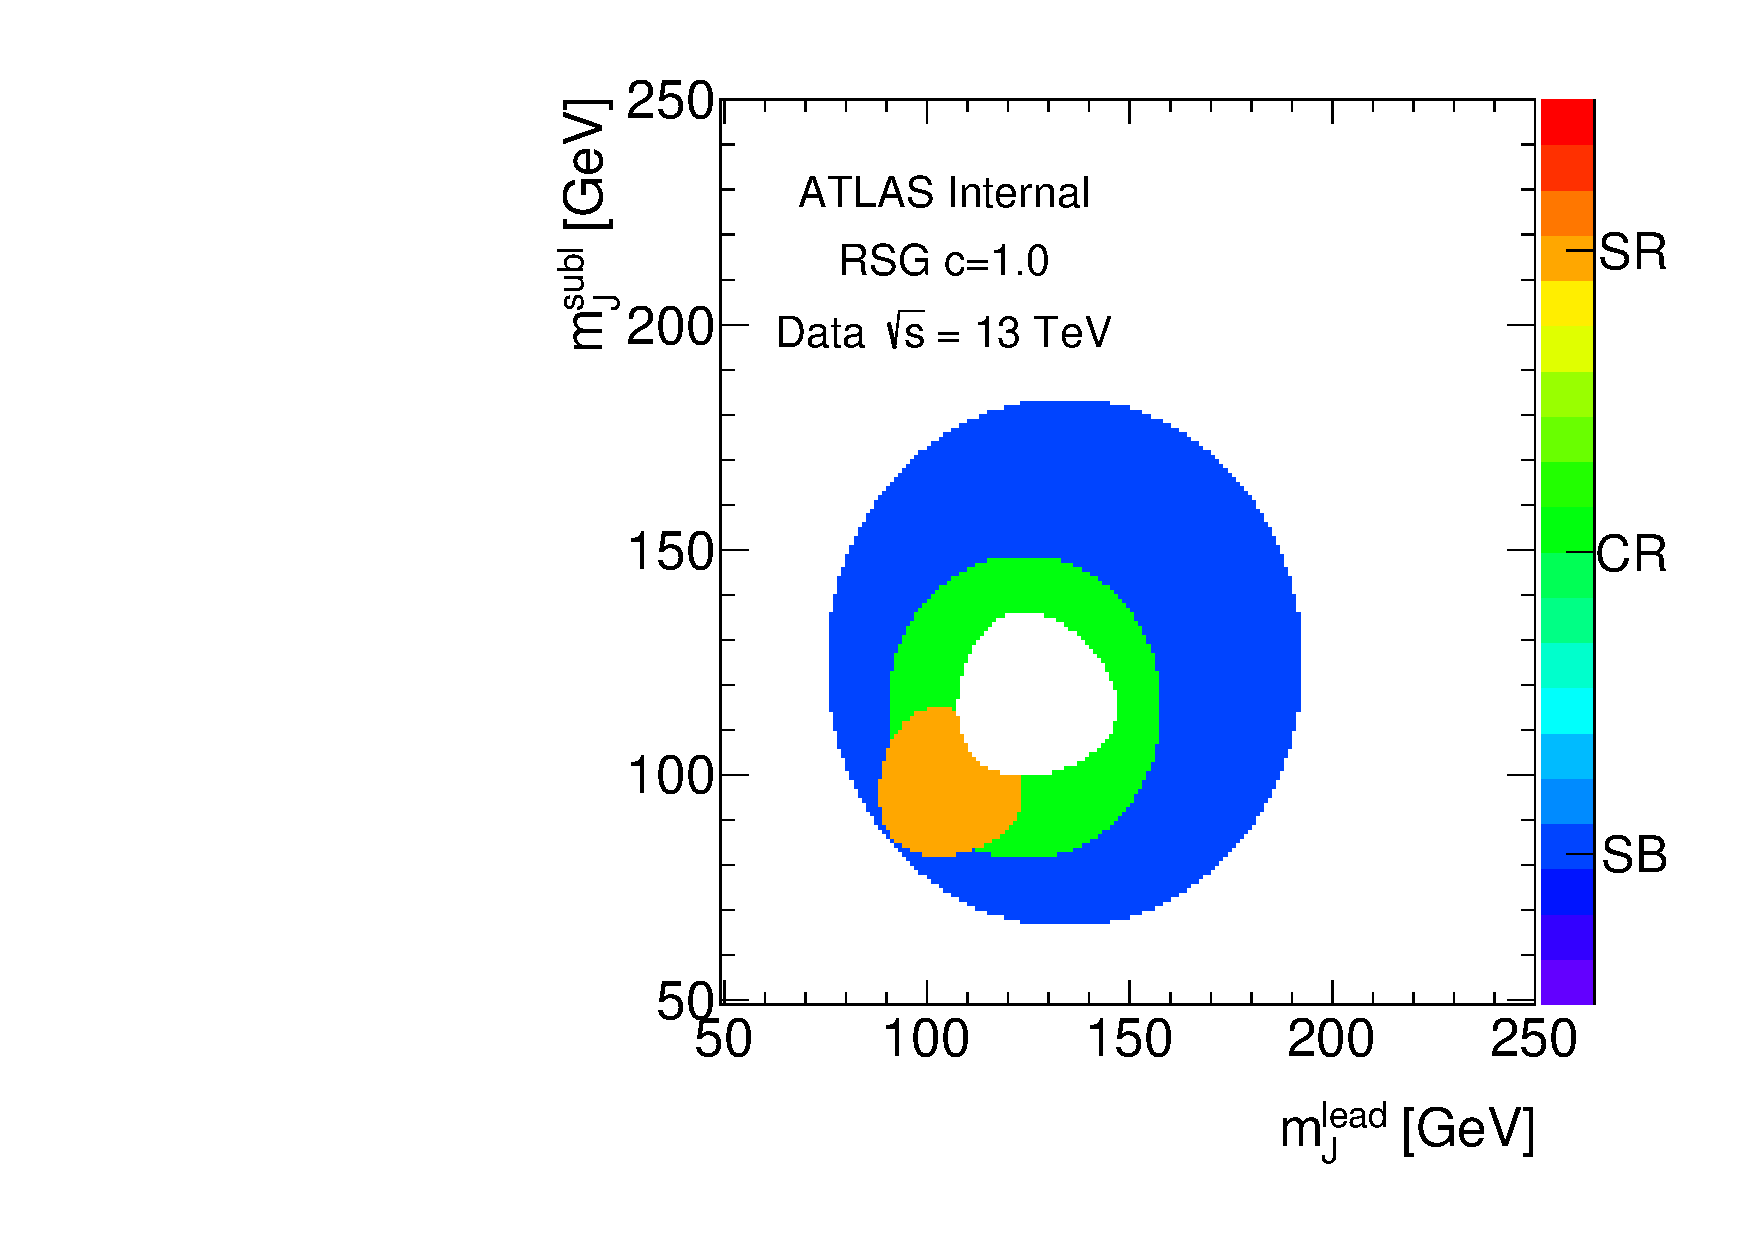
\includegraphics[width=0.4\textwidth,angle=-90]{figures/boosted/ZZ/Compare_NoTag_mH0H1.pdf}
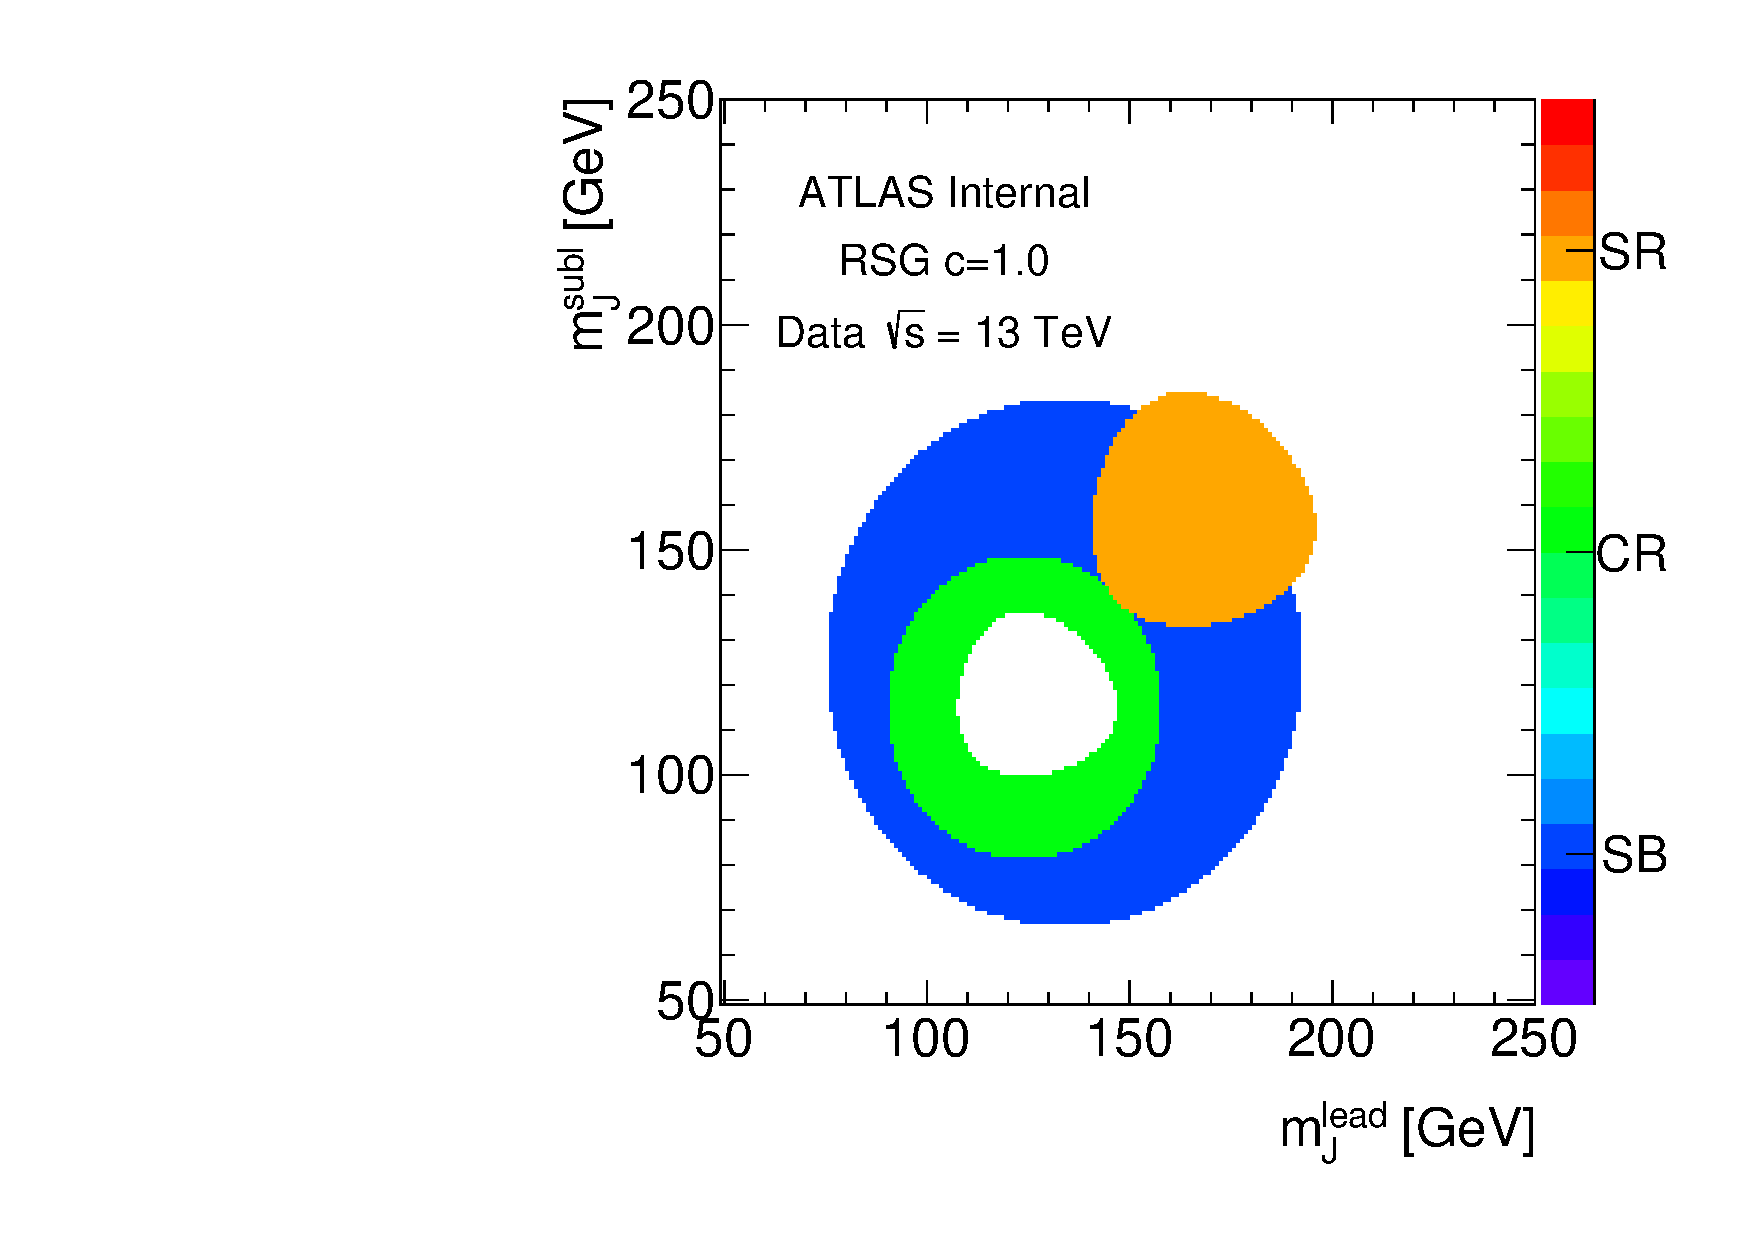
\includegraphics[width=0.4\textwidth,angle=-90]{figures/boosted/TT/Compare_NoTag_mH0H1.pdf}
\end{center}
\caption{Illustration of ZZ (left) and TT (right) signal region as shown in the orange shaded region. Control region shown in green, and Sideband region in blue. The white circle in the midde is the real Signal region, and it is blinded.}
\label{CRSB:ZZIllustration}
\end{figure}

%%\paragraph{}
The summary of background estimation for ZZ signal region can be found in Table \ref{CRSB:SummaryTable_ZZ_4b}, ~\ref{CRSB:SummaryTable_ZZ_3b} and ~\ref{CRSB:SummaryTable_ZZ_2b}. The difference between data and prediction in ZZ signal region is summarized in Table \ref{CRSB:DataPred_ZZSR} for all the regions. The discrepancy between data and prediction is either covered by statistical uncertainty of data or comparable with data statistical uncertainty in 4$b$, 3$b$ and 2$b$s ZZ SR respectively. We further check the kinematic distribution between data and prediction in ZZ SR, as shown in Figure \ref{CRSB:ZZSR_Distribution}. The data agrees with prediction well in general, though a few bins might not agree perfectly. The difference from 4$b$ CR region test is 17$\%$, which is smaller than the 4$b$ ZZ region difference. But the statistical uncertainty in ZZ region (yield 37) is much higher compared with our CR regions (min yield 76), hence the CR region with more statistical power is still used for the non-closure uncertainty.

%%\paragraph{}
The summary of background estimation for TT signal region can be found in Table \ref{CRSB:SummaryTable_TT_4b}, ~\ref{CRSB:SummaryTable_TT_3b} and ~\ref{CRSB:SummaryTable_TT_2b}. The difference between data and prediction in TT signal region is summarized in Table \ref{CRSB:DataPred_TTSR} for all the regions. The discrepancy between data and prediction is either covered by statistical uncertainty of data or comparable with data statistical uncertainty in 4$b$, 3$b$ and 2$b$s TT SR respectively. We further check the kinematic distribution between data and prediction in TT SR, as shown in Figure \ref{CRSB:TTSR_Distribution}. The data agrees with prediction well in general, though a few bins might not agree perfectly. 

%%\paragraph{}
Based on all the variation tests done above, we think there is no need to introduce extra uncertainty on non-closure systematics since most of the data/prediction disagreements are well covered by the data statistical uncertainty.

\begin{table}[htbp!]
\begin{center}
\begin{footnotesize} 
\begin{tabular}{c|c|c|c} 
FourTag & Sideband & Control & Signal \\ 
\hline\hline 
QCD Est & 166.65 $\pm$ 2.88 & 45.83 $\pm$ 1.51 & 27.37 $\pm$ 1.16\\ 
$t\bar{t}$ Est.  & 27.52 $\pm$ 0.25 & 6.31 $\pm$ 0.14 & 0 $\pm$ 0\\ 
$Z+jets$ & 0 $\pm$ 0 & 6.18 $\pm$ 5.12 & 0 $\pm$ 0\\ 
Total Bkg Est & 194.17 $\pm$ 2.89 & 58.32 $\pm$ 5.34 & 27.37 $\pm$ 1.16\\ 
Data & 194.0 $\pm$ 13.93 & 54.0 $\pm$ 7.35 & 37.0 $\pm$ 6.08\\ 
$c=1.0$,$m=1.0TeV$ & 2.45 $\pm$ 0.098 & 4.47 $\pm$ 0.13 & 0.99 $\pm$ 0.063\\ 
$c=1.0$,$m=2.0TeV$ & 0.032 $\pm$ 0.0015 & 0.075 $\pm$ 0.0022 & 0.028 $\pm$ 0.0014\\ 
$c=1.0$,$m=3.0TeV$ & 0.00029 $\pm$ 3.5e-05 & 0.00064 $\pm$ 5e-05 & 0.0002 $\pm$ 2.7e-05\\ 
\hline\hline 
\end{tabular} 
\end{footnotesize} 
\newline 

\end{center}
\caption{Background prediction in SR/CR/SB for ZZ SR in 4$b$-tag region. Uncertainties are stat only.}
\label{CRSB:SummaryTable_ZZ_4b}
\end{table}

\begin{table}[htbp!]
\begin{center}
\begin{footnotesize} 
\begin{tabular}{c|c|c|c} 
ThreeTag & Sideband & Control & Signal \\ 
\hline\hline 
& & & \\ 
QCD Est & 3344.46 $\pm$ 26.85 & 998.41 $\pm$ 14.63 & 637.78 $\pm$ 11.87\\ 
$t\bar{t}$ Est.  & 826.66 $\pm$ 25.11 & 136.58 $\pm$ 10.23 & 30.07 $\pm$ 1.24\\ 
$Z+jets$ & 32.49 $\pm$ 11.34 & 8.22 $\pm$ 5.29 & 3.3 $\pm$ 2.0\\ 
Total Bkg Est & 4203.61 $\pm$ 38.47 & 1143.2 $\pm$ 18.62 & 671.15 $\pm$ 12.11\\ 
Data & 4203.0 $\pm$ 64.83 & 1108.0 $\pm$ 33.29 & 645.0 $\pm$ 25.4\\ 
$c=1.0$,$m=1.0TeV$ & 7.56 $\pm$ 0.18 & 9.84 $\pm$ 0.2 & 3.05 $\pm$ 0.11\\ 
$c=1.0$,$m=2.0TeV$ & 0.15 $\pm$ 0.0033 & 0.27 $\pm$ 0.0046 & 0.12 $\pm$ 0.003\\ 
$c=1.0$,$m=3.0TeV$ & 0.0034 $\pm$ 0.00012 & 0.0056 $\pm$ 0.00016 & 0.0021 $\pm$ 9.5e-05\\ 
& & & \\ 
\hline\hline 
\end{tabular} 
\end{footnotesize} 
\newline 

\end{center}
\caption{Background prediction in SR/CR/SB for ZZ SR in 3$b$-tag region. Uncertainties are stat only.}
\label{CRSB:SummaryTable_ZZ_3b}
\end{table}

\begin{table}[htbp!]
\begin{center}
\begin{footnotesize} 
\begin{tabular}{c|c|c|c} 
TwoTag split & Sideband & Control & Signal \\ 
\hline\hline 
QCD Est & 16387.44 $\pm$ 37.6 & 4827.76 $\pm$ 19.86 & 3026.83 $\pm$ 15.61\\ 
$t\bar{t}$ Est.  & 7671.95 $\pm$ 69.14 & 1229.96 $\pm$ 26.54 & 332.29 $\pm$ 13.66\\ 
$Z+jets$ & 44.37 $\pm$ 13.23 & 13.34 $\pm$ 6.6 & 36.47 $\pm$ 12.88\\ 
Total Bkg Est & 24103.77 $\pm$ 79.8 & 6071.07 $\pm$ 33.8 & 3395.59 $\pm$ 24.42\\ 
Data & 24104.0 $\pm$ 155.25 & 6261.0 $\pm$ 79.13 & 3258.0 $\pm$ 57.08\\ 
$c=1.0$,$m=1.0TeV$ & 4.57 $\pm$ 0.14 & 4.65 $\pm$ 0.14 & 1.91 $\pm$ 0.089\\ 
$c=1.0$,$m=2.0TeV$ & 0.16 $\pm$ 0.0038 & 0.26 $\pm$ 0.0047 & 0.12 $\pm$ 0.0032\\ 
$c=1.0$,$m=3.0TeV$ & 0.012 $\pm$ 0.00024 & 0.019 $\pm$ 0.00029 & 0.0085 $\pm$ 0.00019\\ 
\hline\hline 
\end{tabular} 
\end{footnotesize} 
\newline 

\end{center}
\caption{Background prediction in SR/CR/SB for ZZ SR in 2$b$s-tag region. Uncertainties are stat only.}
\label{CRSB:SummaryTable_ZZ_2b}
\end{table}

\begin{table}[htbp!]
\begin{center}
\begin{footnotesize} 
\begin{tabular}{c|c|c|c} 
ZZ Signal Region & Data & Prediction & (Predict - Data)/Data \\ 
\hline\hline 
FourTag & 37.0 $\pm$ 6.08 & 27.37 $\pm$ 1.16 & -26.0 $\%$  $\pm$ 15.3 $\%$ \\ 
\hline 
ThreeTag & 645.0 $\pm$ 25.4 & 671.15 $\pm$ 12.11 & 4.05 $\%$  $\pm$ 5.97 $\%$ \\ 
\hline 
TwoTag split & 3258.0 $\pm$ 57.08 & 3395.59 $\pm$ 24.42 & 4.22 $\%$  $\pm$ 2.58 $\%$ \\ 
\hline\hline 
\end{tabular} 
\end{footnotesize} 
\newline 

\end{center}
\caption{Agreement between data and prediction in ZZ SR in 4$b$, 3$b$ and 2$b$s regions.}
\label{CRSB:DataPred_ZZSR}
\end{table}

\begin{figure}[htbp!]
\begin{center}
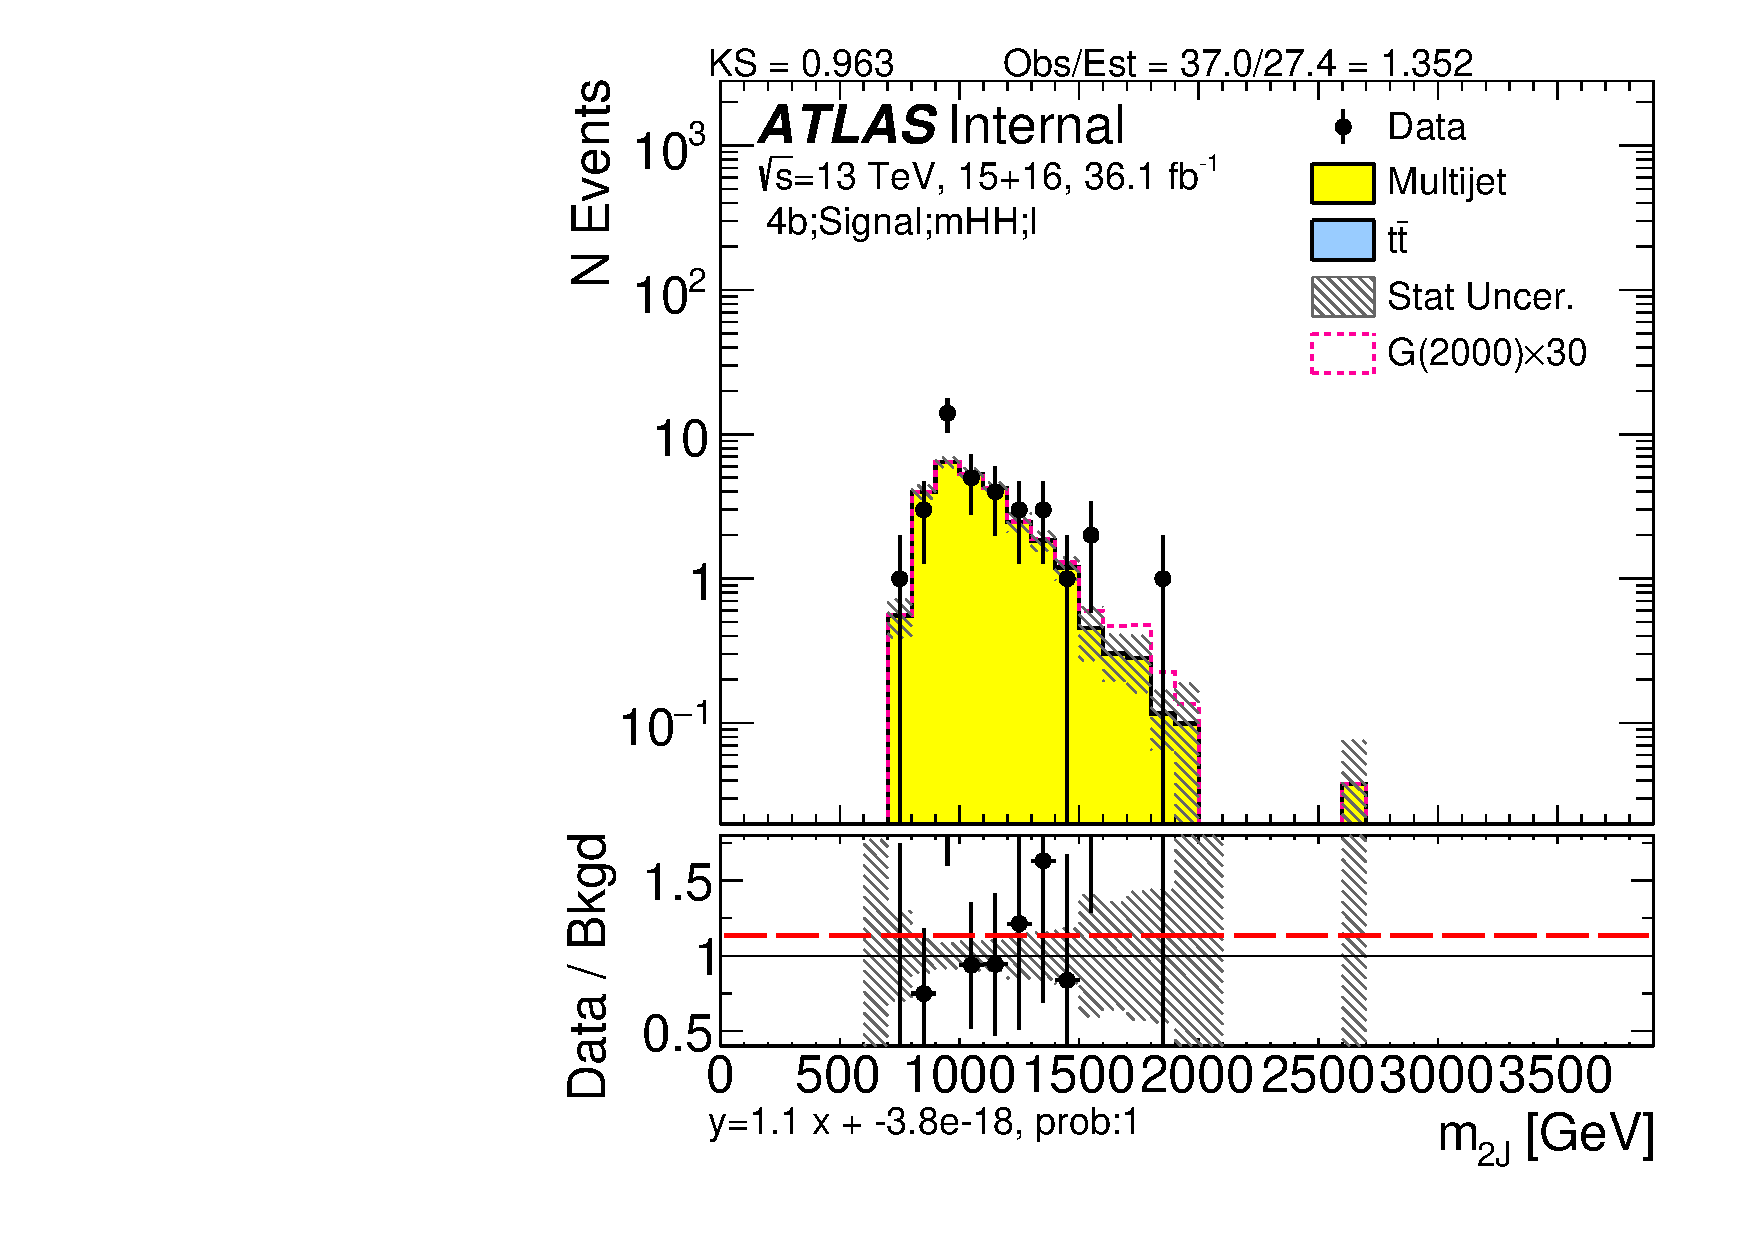
\includegraphics[width=0.45\textwidth,angle=-90]{figures/boosted/ZZ/Moriond_ZZ_FourTag_Signal_mHH_l_1.pdf}
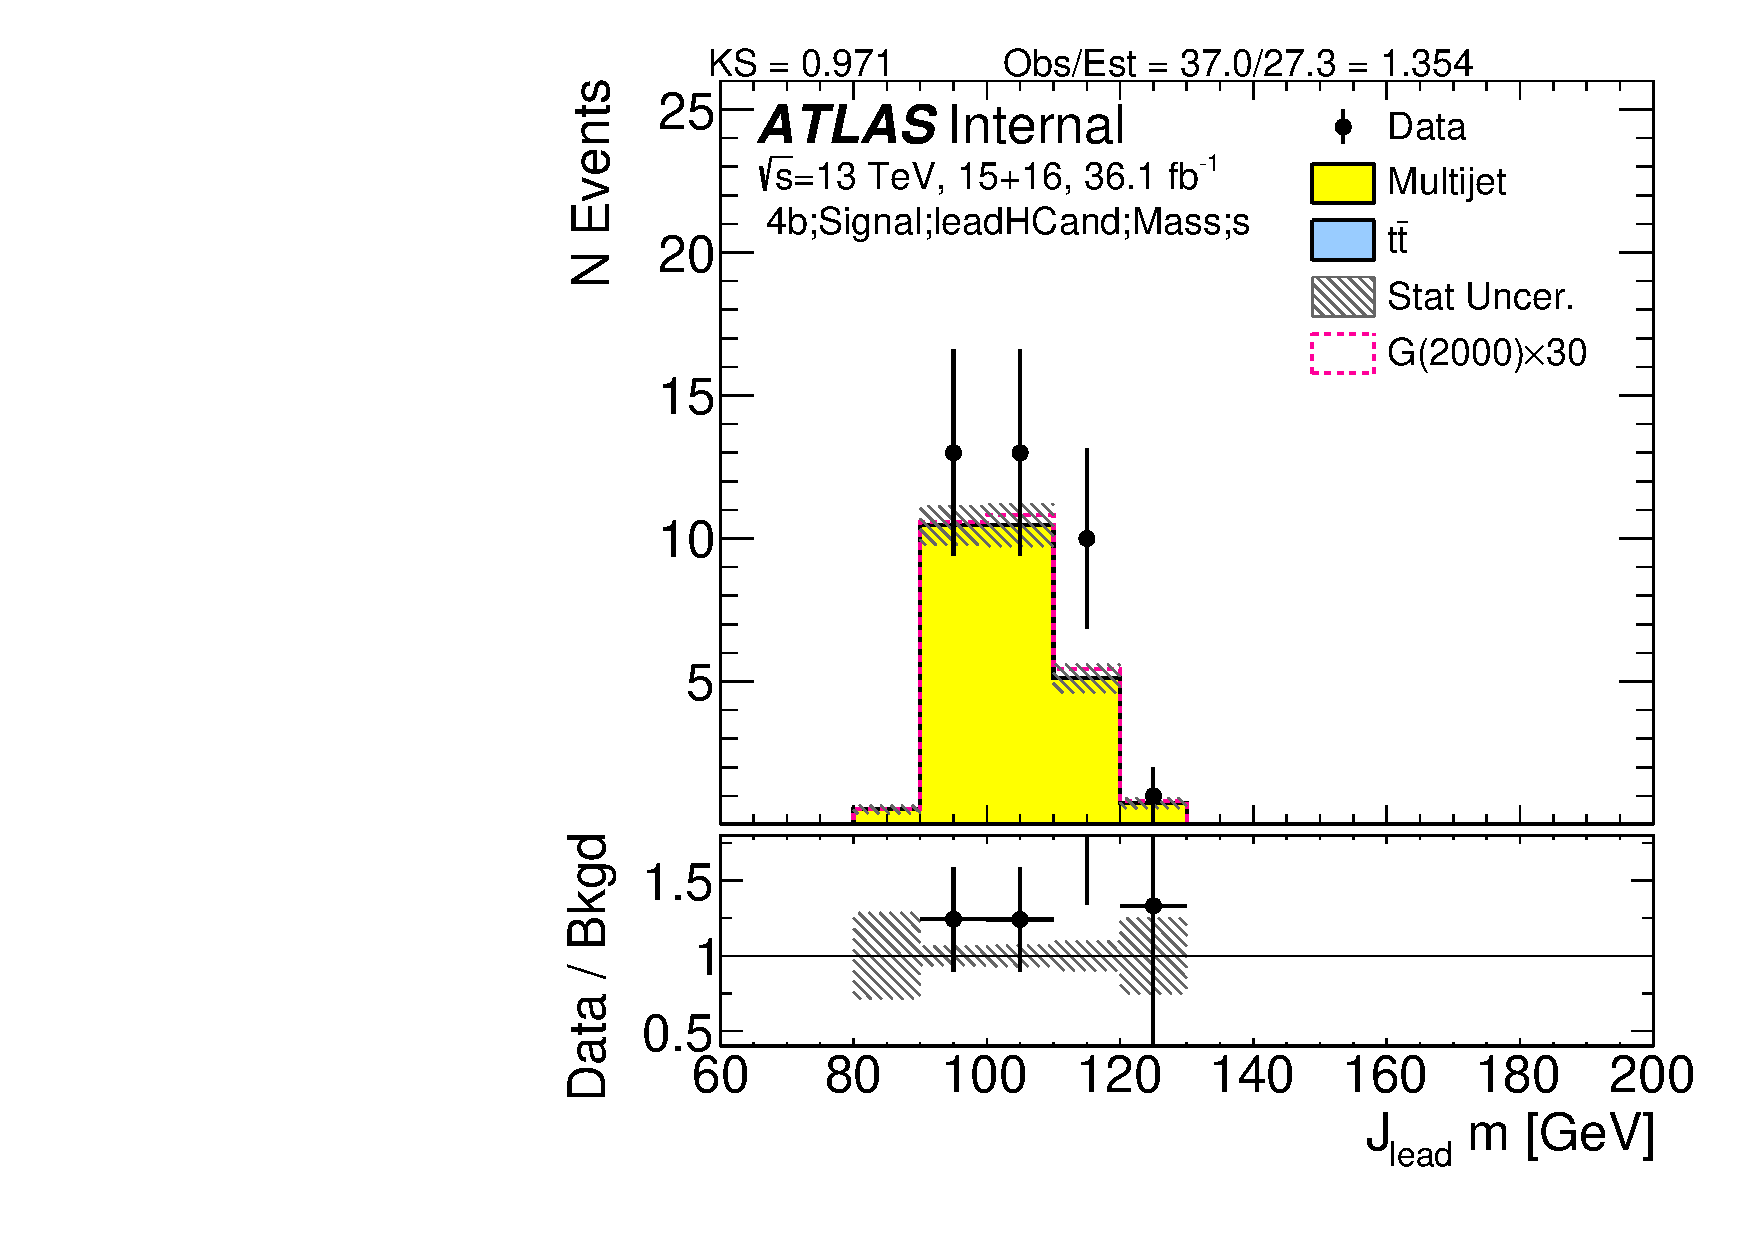
\includegraphics[width=0.45\textwidth,angle=-90]{figures/boosted/ZZ/Moriond_ZZ_FourTag_Signal_leadHCand_Mass_s.pdf}\\
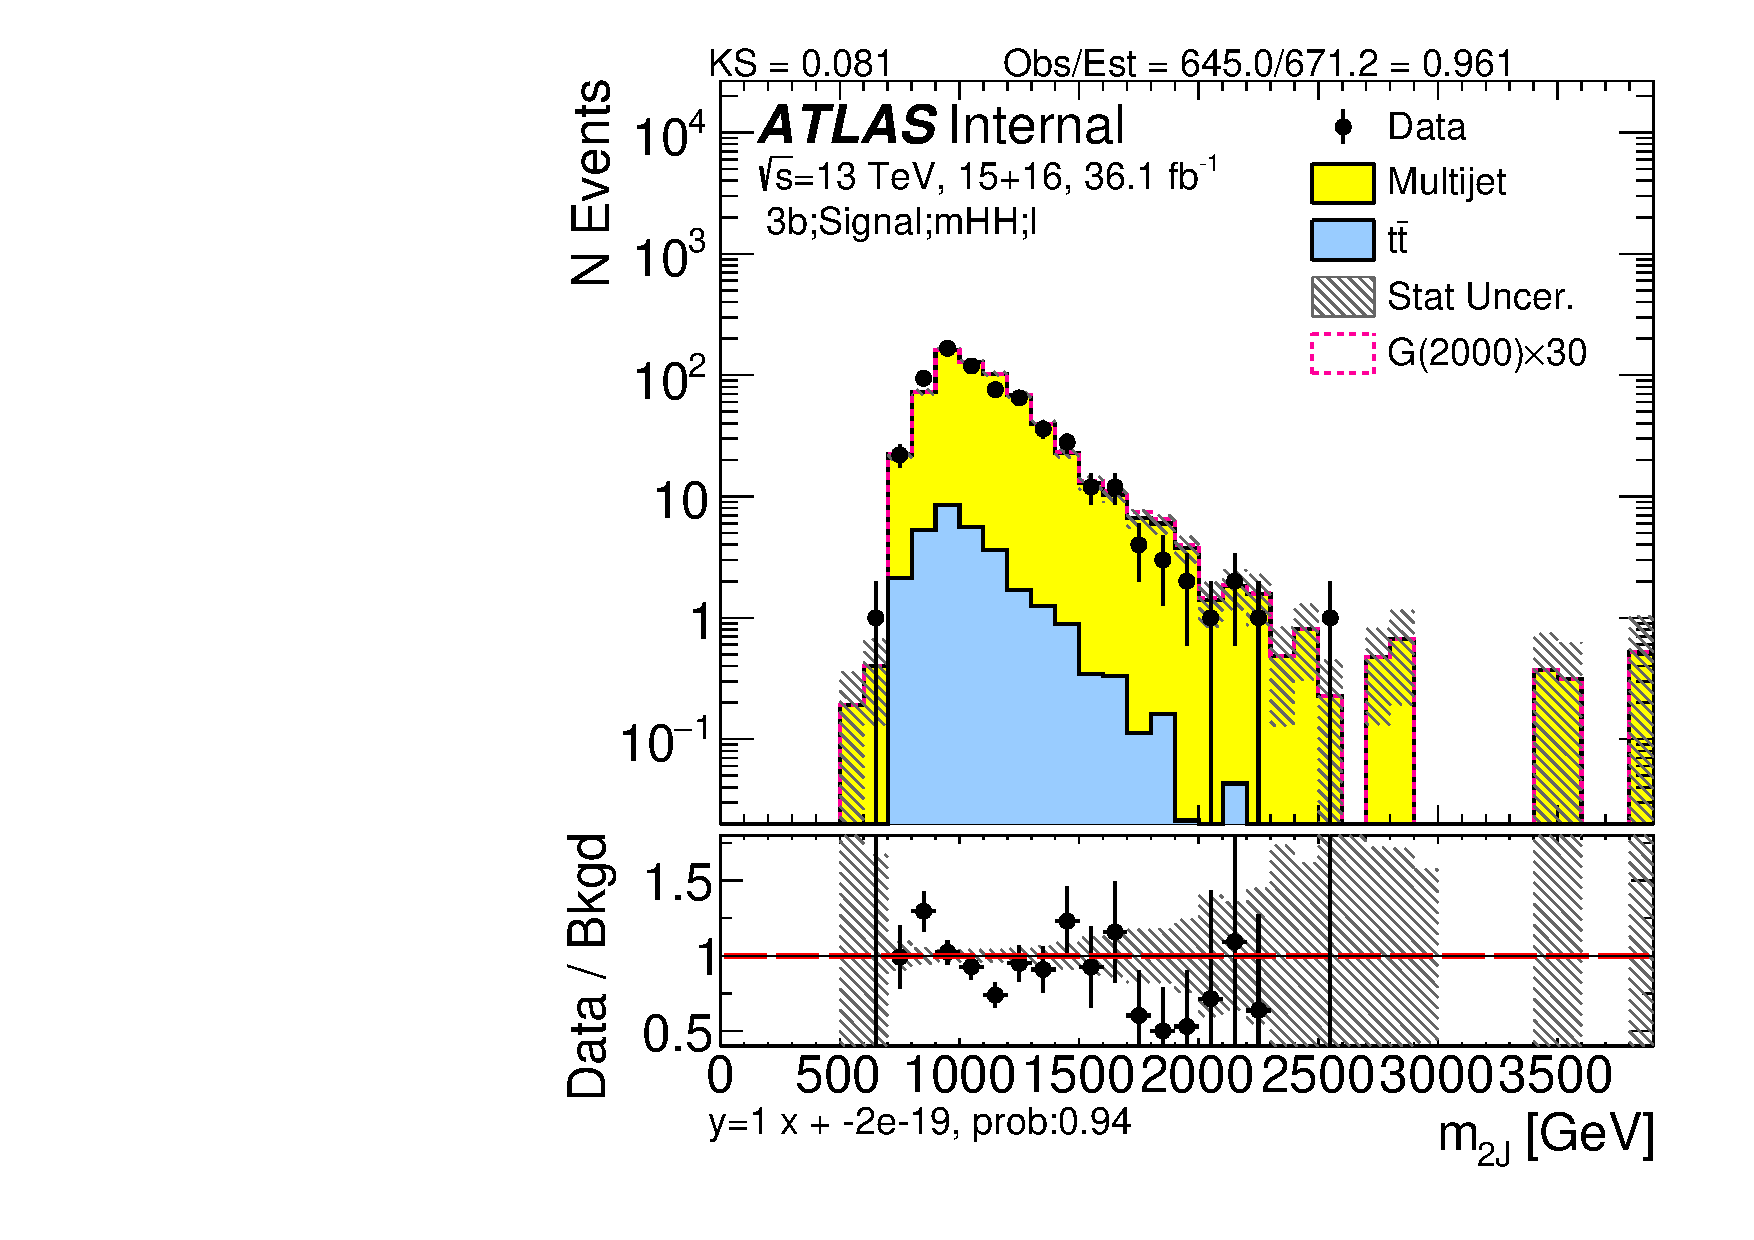
\includegraphics[width=0.45\textwidth,angle=-90]{figures/boosted/ZZ/Moriond_ZZ_ThreeTag_Signal_mHH_l_1.pdf}
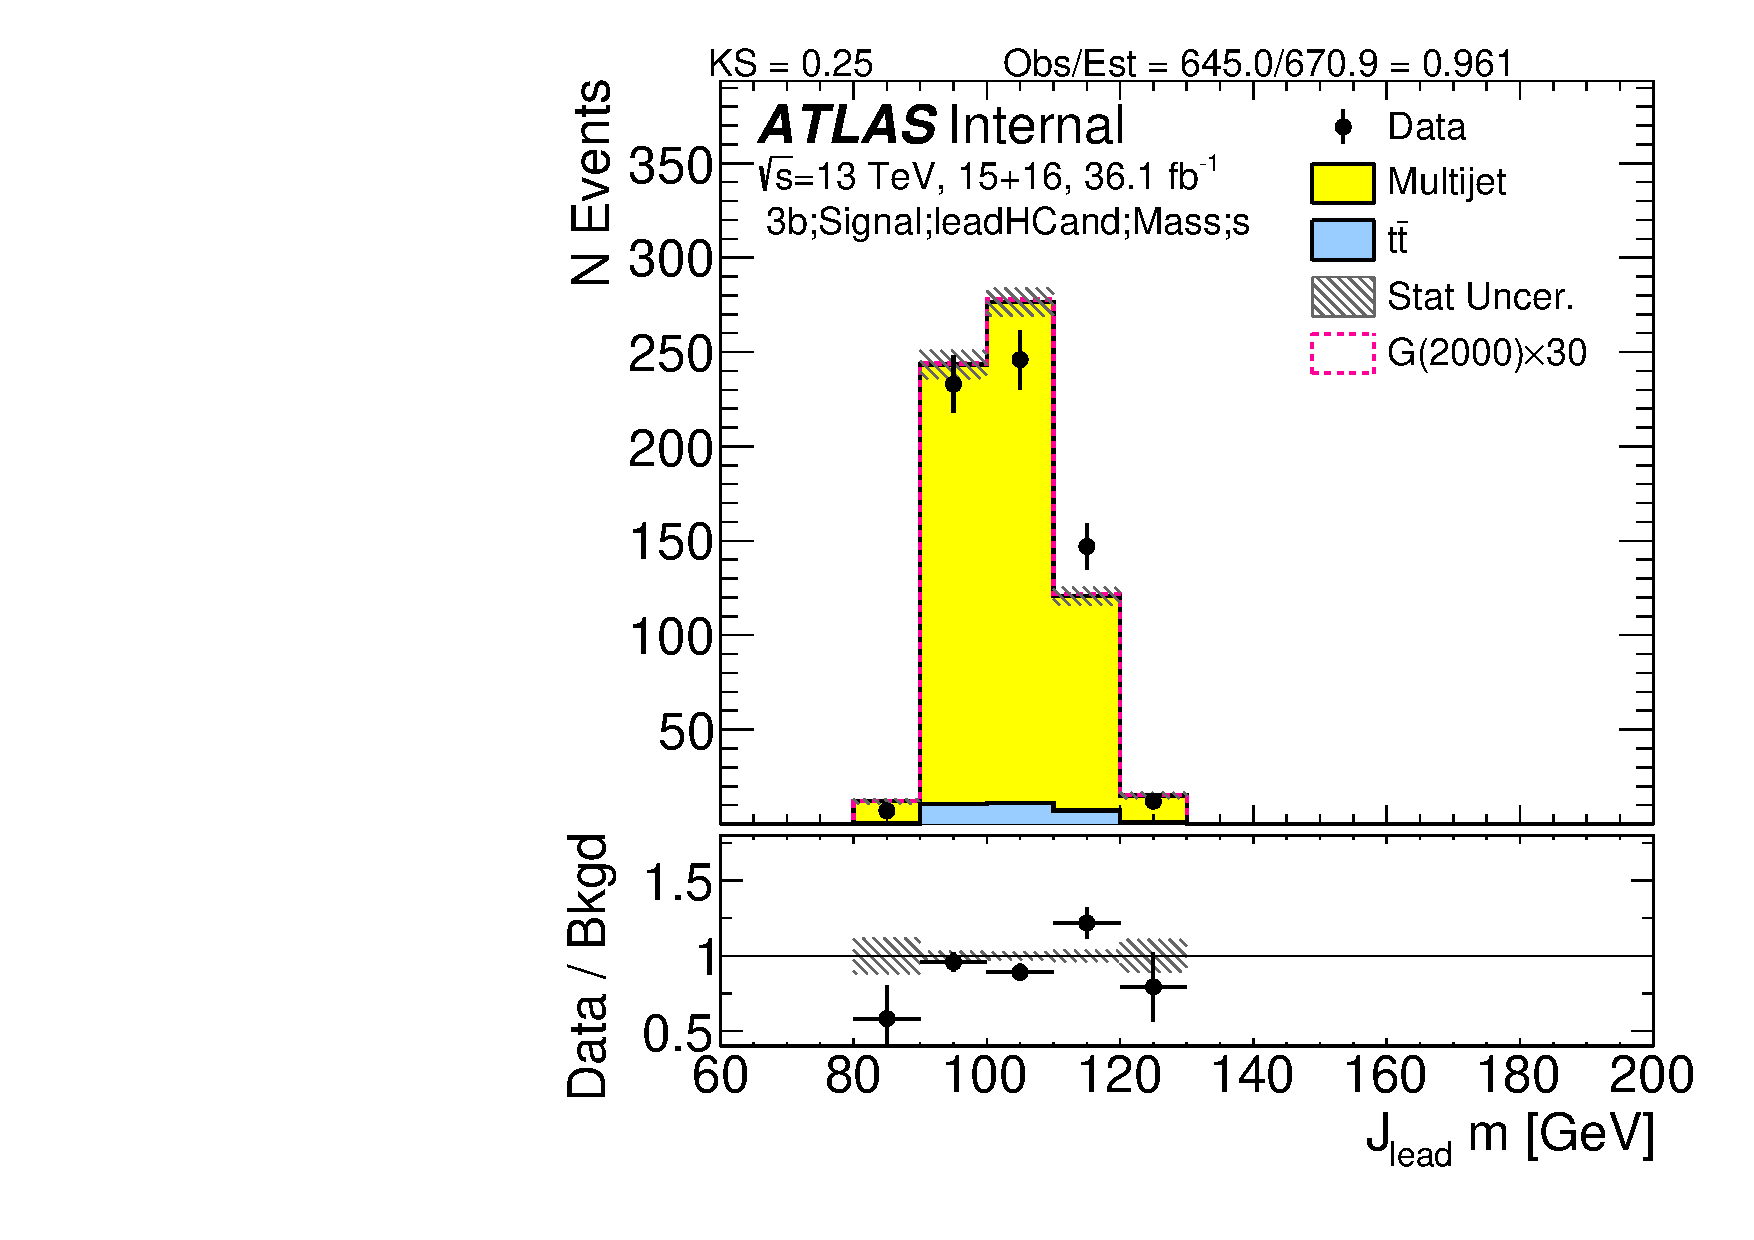
\includegraphics[width=0.45\textwidth,angle=-90]{figures/boosted/ZZ/Moriond_ZZ_ThreeTag_Signal_leadHCand_Mass_s.pdf}\\
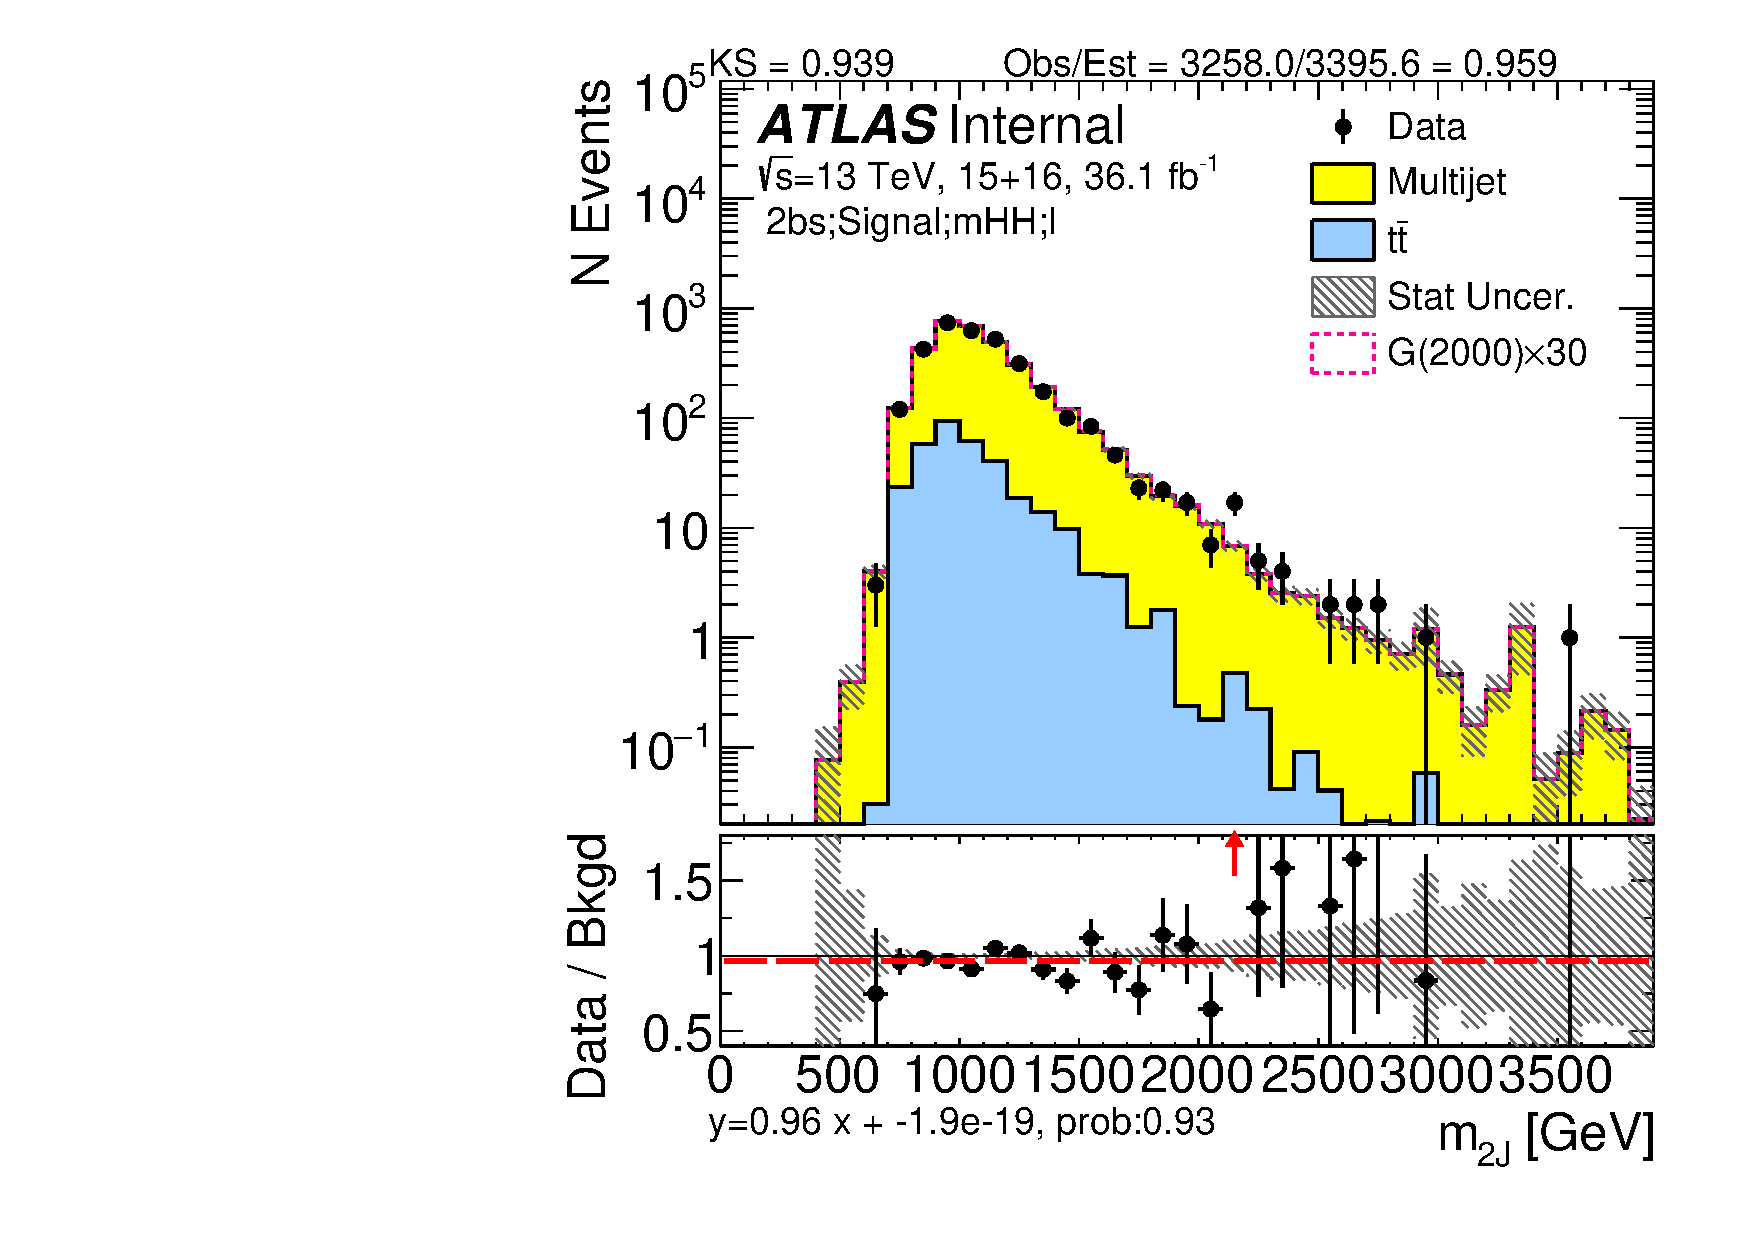
\includegraphics[width=0.45\textwidth,angle=-90]{figures/boosted/ZZ/Moriond_ZZ_TwoTag_split_Signal_mHH_l_1.pdf}
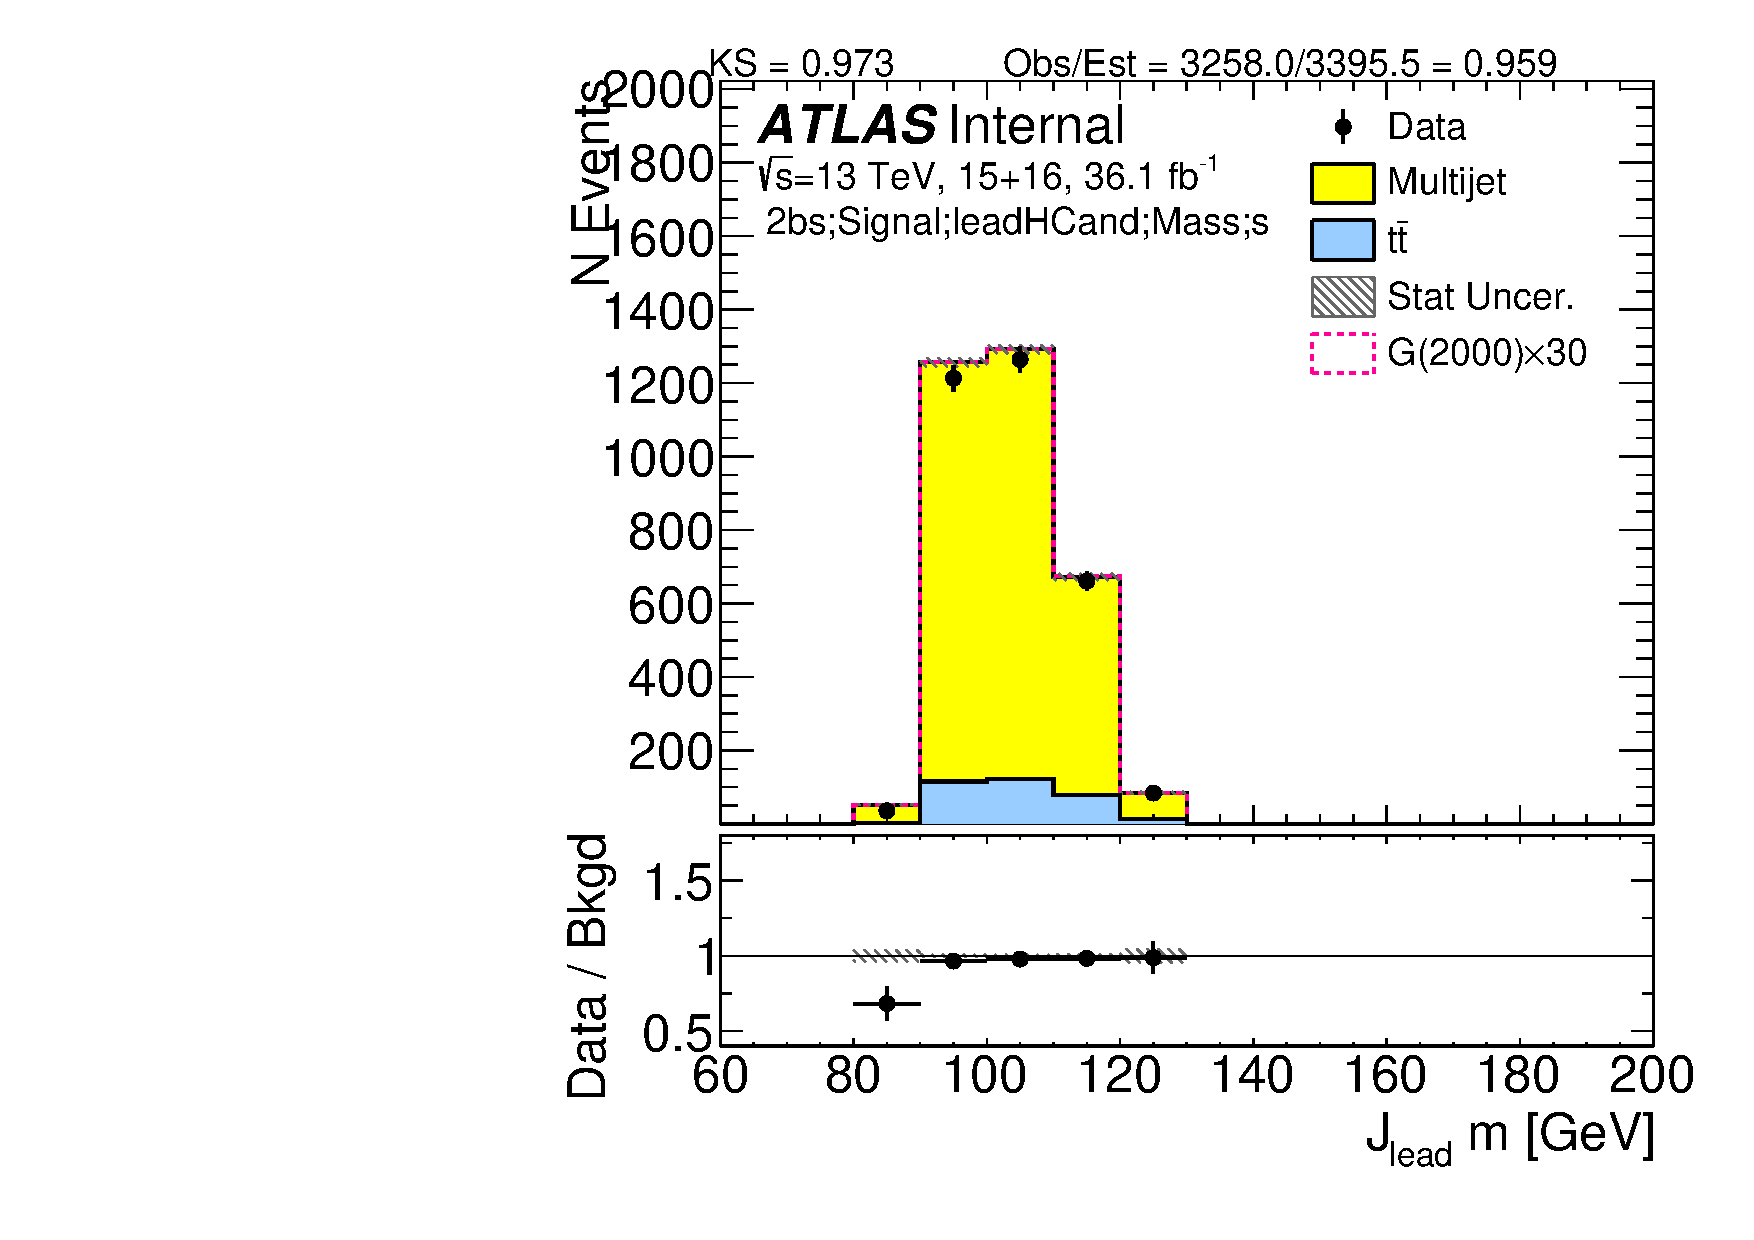
\includegraphics[width=0.45\textwidth,angle=-90]{figures/boosted/ZZ/Moriond_ZZ_TwoTag_split_Signal_leadHCand_Mass_s.pdf}\\
\end{center}
\caption{ZZ signal region distribution of di-jet mass (left column) and leading large-R jet mass (right column) in low mass signal, for 4$b$ (top row), 3$b$(middle row) and 2$b$ split (bottom row). The plots are with only statistical uncertainty.}
\label{CRSB:ZZSR_Distribution}
\end{figure}

\begin{table}[htbp!]
\begin{center}
\begin{footnotesize} 
\begin{tabular}{c|c|c|c} 
FourTag & Sideband & Control & Signal \\ 
\hline\hline 
& & & \\ 
QCD Est & 152.28 $\pm$ 2.72 & 63.47 $\pm$ 1.77 & 28.6 $\pm$ 1.21\\ 
$t\bar{t}$ Est.  & 19.86 $\pm$ 0.22 & 7.45 $\pm$ 0.15 & 15.02 $\pm$ 0.2\\ 
$Z+jets$ & 0 $\pm$ 0 & 6.18 $\pm$ 5.12 & 0 $\pm$ 0\\ 
Total Bkg Est & 172.14 $\pm$ 2.73 & 77.1 $\pm$ 5.42 & 43.62 $\pm$ 1.23\\ 
Data & 172.0 $\pm$ 13.11 & 81.0 $\pm$ 9.0 & 46.0 $\pm$ 6.78\\ 
$c=1.0$,$m=1.0TeV$ & 2.38 $\pm$ 0.097 & 5.4 $\pm$ 0.15 & 0.15 $\pm$ 0.024\\ 
$c=1.0$,$m=2.0TeV$ & 0.033 $\pm$ 0.0015 & 0.1 $\pm$ 0.0026 & 0.0011 $\pm$ 0.00027\\ 
$c=1.0$,$m=3.0TeV$ & 0.00031 $\pm$ 3.6e-05 & 0.0008 $\pm$ 5.6e-05 & 1.5e-05 $\pm$ 7.7e-06\\ 
& & & \\ 
\hline\hline 
\end{tabular} 
\end{footnotesize} 
\newline 

\end{center}
\caption{Background prediction in SR/CR/SB for TT SR in 4$b$-tag region. Uncertainties are stat only.}
\label{CRSB:SummaryTable_TT_4b}
\end{table}

\begin{table}[htbp!]
\begin{center}
\begin{footnotesize} 
\begin{tabular}{c|c|c|c} 
ThreeTag & Sideband & Control & Signal \\ 
\hline\hline 
QCD Est & 3106.11 $\pm$ 25.79 & 1427.41 $\pm$ 17.53 & 570.01 $\pm$ 11.6\\ 
$t\bar{t}$ Est.  & 495.21 $\pm$ 18.75 & 148.55 $\pm$ 10.21 & 406.57 $\pm$ 5.42\\ 
$Z+jets$ & 32.5 $\pm$ 11.34 & 11.21 $\pm$ 5.65 & 0.3 $\pm$ 0.3\\ 
Total Bkg Est & 3633.82 $\pm$ 33.85 & 1587.17 $\pm$ 21.05 & 976.88 $\pm$ 12.81\\ 
Data & 3633.0 $\pm$ 60.27 & 1553.0 $\pm$ 39.41 & 1017.0 $\pm$ 31.89\\ 
$c=1.0$,$m=1.0TeV$ & 7.57 $\pm$ 0.18 & 12.58 $\pm$ 0.23 & 0.32 $\pm$ 0.037\\ 
$c=1.0$,$m=2.0TeV$ & 0.15 $\pm$ 0.0034 & 0.38 $\pm$ 0.0054 & 0.0047 $\pm$ 0.0006\\ 
$c=1.0$,$m=3.0TeV$ & 0.0034 $\pm$ 0.00012 & 0.0075 $\pm$ 0.00018 & 0.00023 $\pm$ 3.3e-05\\ 
\hline\hline 
\end{tabular} 
\end{footnotesize} 
\newline 

\end{center}
\caption{Background prediction in SR/CR/SB for TT SR in 3$b$-tag region. Uncertainties are stat only.}
\label{CRSB:SummaryTable_TT_3b}
\end{table}

\begin{table}[htbp!]
\begin{center}
\begin{footnotesize} 
\begin{tabular}{c|c|c|c} 
TwoTag split & Sideband & Control & Signal \\ 
\hline\hline 
QCD Est & 14980.05 $\pm$ 35.33 & 6803.06 $\pm$ 23.41 & 2817.92 $\pm$ 16.54\\ 
$t\bar{t}$ Est.  & 5170.92 $\pm$ 56.22 & 1468.85 $\pm$ 28.93 & 3628.91 $\pm$ 48.42\\ 
$Z+jets$ & 61.34 $\pm$ 16.04 & 26.44 $\pm$ 10.08 & 6.4 $\pm$ 5.05\\ 
Total Bkg Est & 20212.31 $\pm$ 68.31 & 8298.34 $\pm$ 38.56 & 6453.23 $\pm$ 51.41\\ 
Data & 20212.0 $\pm$ 142.17 & 8486.0 $\pm$ 92.12 & 6446.0 $\pm$ 80.29\\ 
$c=1.0$,$m=1.0TeV$ & 4.59 $\pm$ 0.14 & 6.33 $\pm$ 0.16 & 0.24 $\pm$ 0.033\\ 
$c=1.0$,$m=2.0TeV$ & 0.17 $\pm$ 0.0039 & 0.36 $\pm$ 0.0056 & 0.0066 $\pm$ 0.00077\\ 
$c=1.0$,$m=3.0TeV$ & 0.012 $\pm$ 0.00024 & 0.027 $\pm$ 0.00034 & 0.00089 $\pm$ 6.7e-05\\ 
\hline\hline 
\end{tabular} 
\end{footnotesize} 
\newline 

\end{center}
\caption{Background prediction in SR/CR/SB for TT SR in 2$b$s-tag region. Uncertainties are stat only.}
\label{CRSB:SummaryTable_TT_2b}
\end{table}

\begin{table}[htbp!]
\begin{center}
\begin{footnotesize} 
\begin{tabular}{c|c|c|c} 
TT Signal Region & Data & Prediction & (Predict - Data)/Data \\ 
\hline\hline 
FourTag & 46.0 $\pm$ 6.78 & 43.62 $\pm$ 1.23 & -5.18 $\%$  $\pm$ 16.66 $\%$ \\ 
\hline 
ThreeTag & 1017.0 $\pm$ 31.89 & 976.88 $\pm$ 12.81 & -3.95 $\%$  $\pm$ 4.27 $\%$ \\ 
\hline 
TwoTag split & 6446.0 $\pm$ 80.29 & 6453.23 $\pm$ 51.41 & 0.11 $\%$  $\pm$ 2.04 $\%$ \\ 
\hline\hline 
\end{tabular} 
\end{footnotesize} 
\newline 

\end{center}
\caption{Agreement between data and prediction in TT SR in 4$b$, 3$b$ and 2$b$s regions.}
\label{CRSB:DataPred_TTSR}
\end{table}


\begin{figure}[htbp!]
\begin{center}
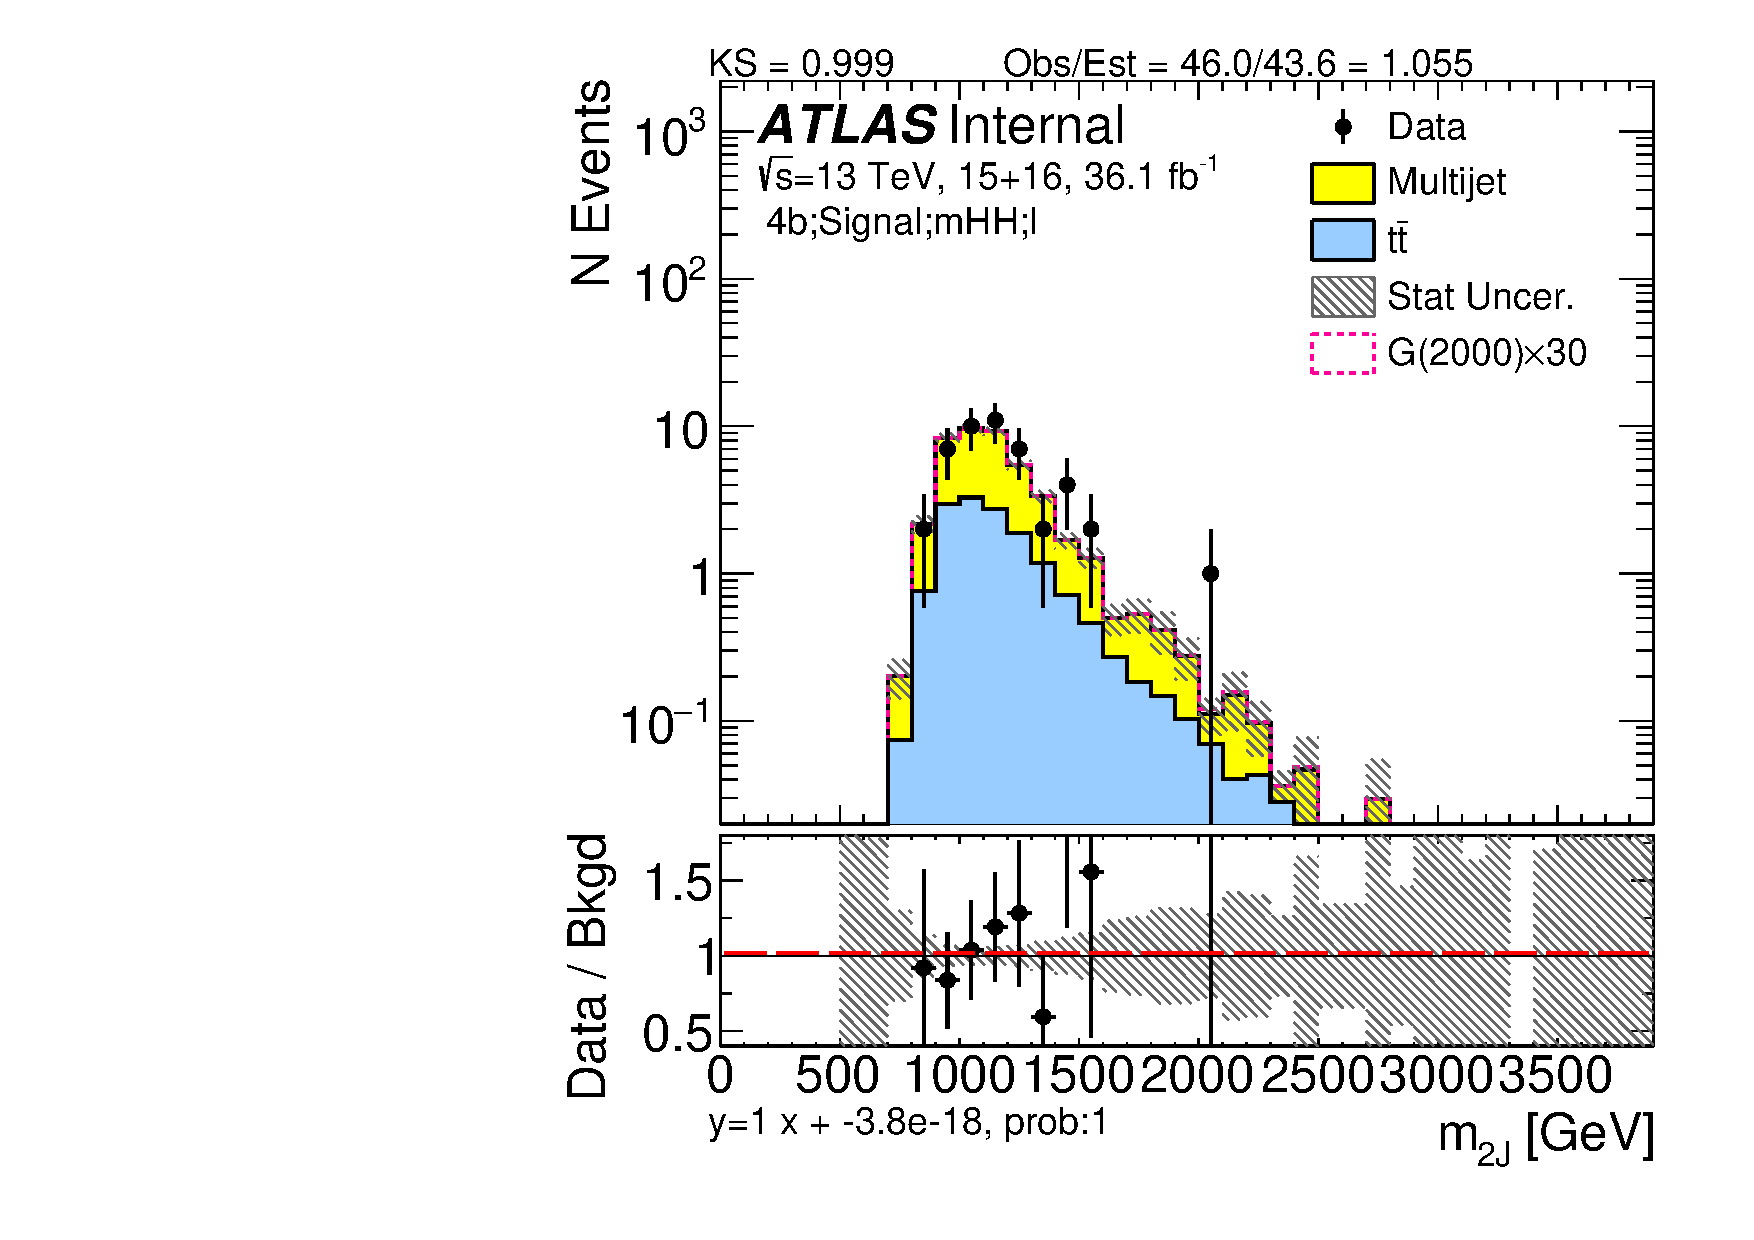
\includegraphics[width=0.45\textwidth,angle=-90]{figures/boosted/TT/Moriond_TT_FourTag_Signal_mHH_l_1.pdf}
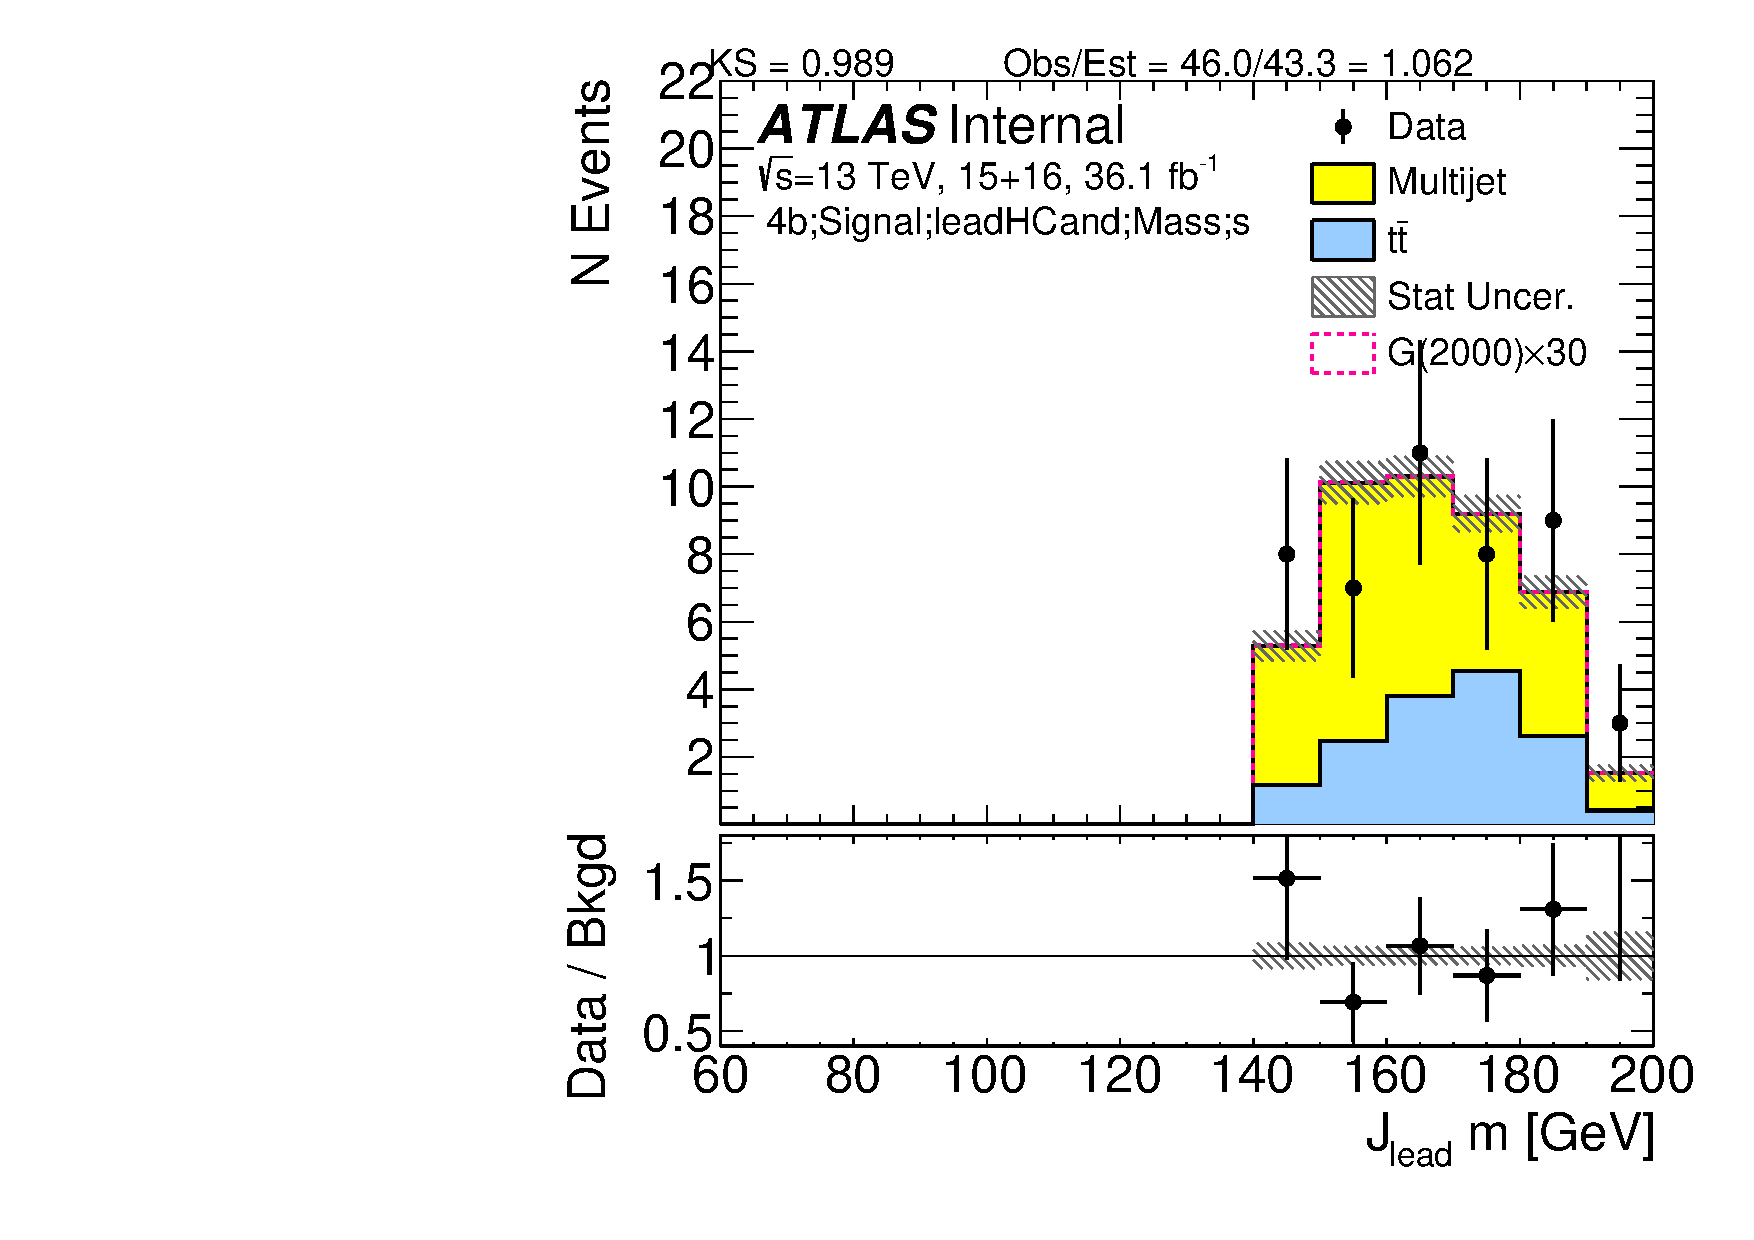
\includegraphics[width=0.45\textwidth,angle=-90]{figures/boosted/TT/Moriond_TT_FourTag_Signal_leadHCand_Mass_s.pdf}\\
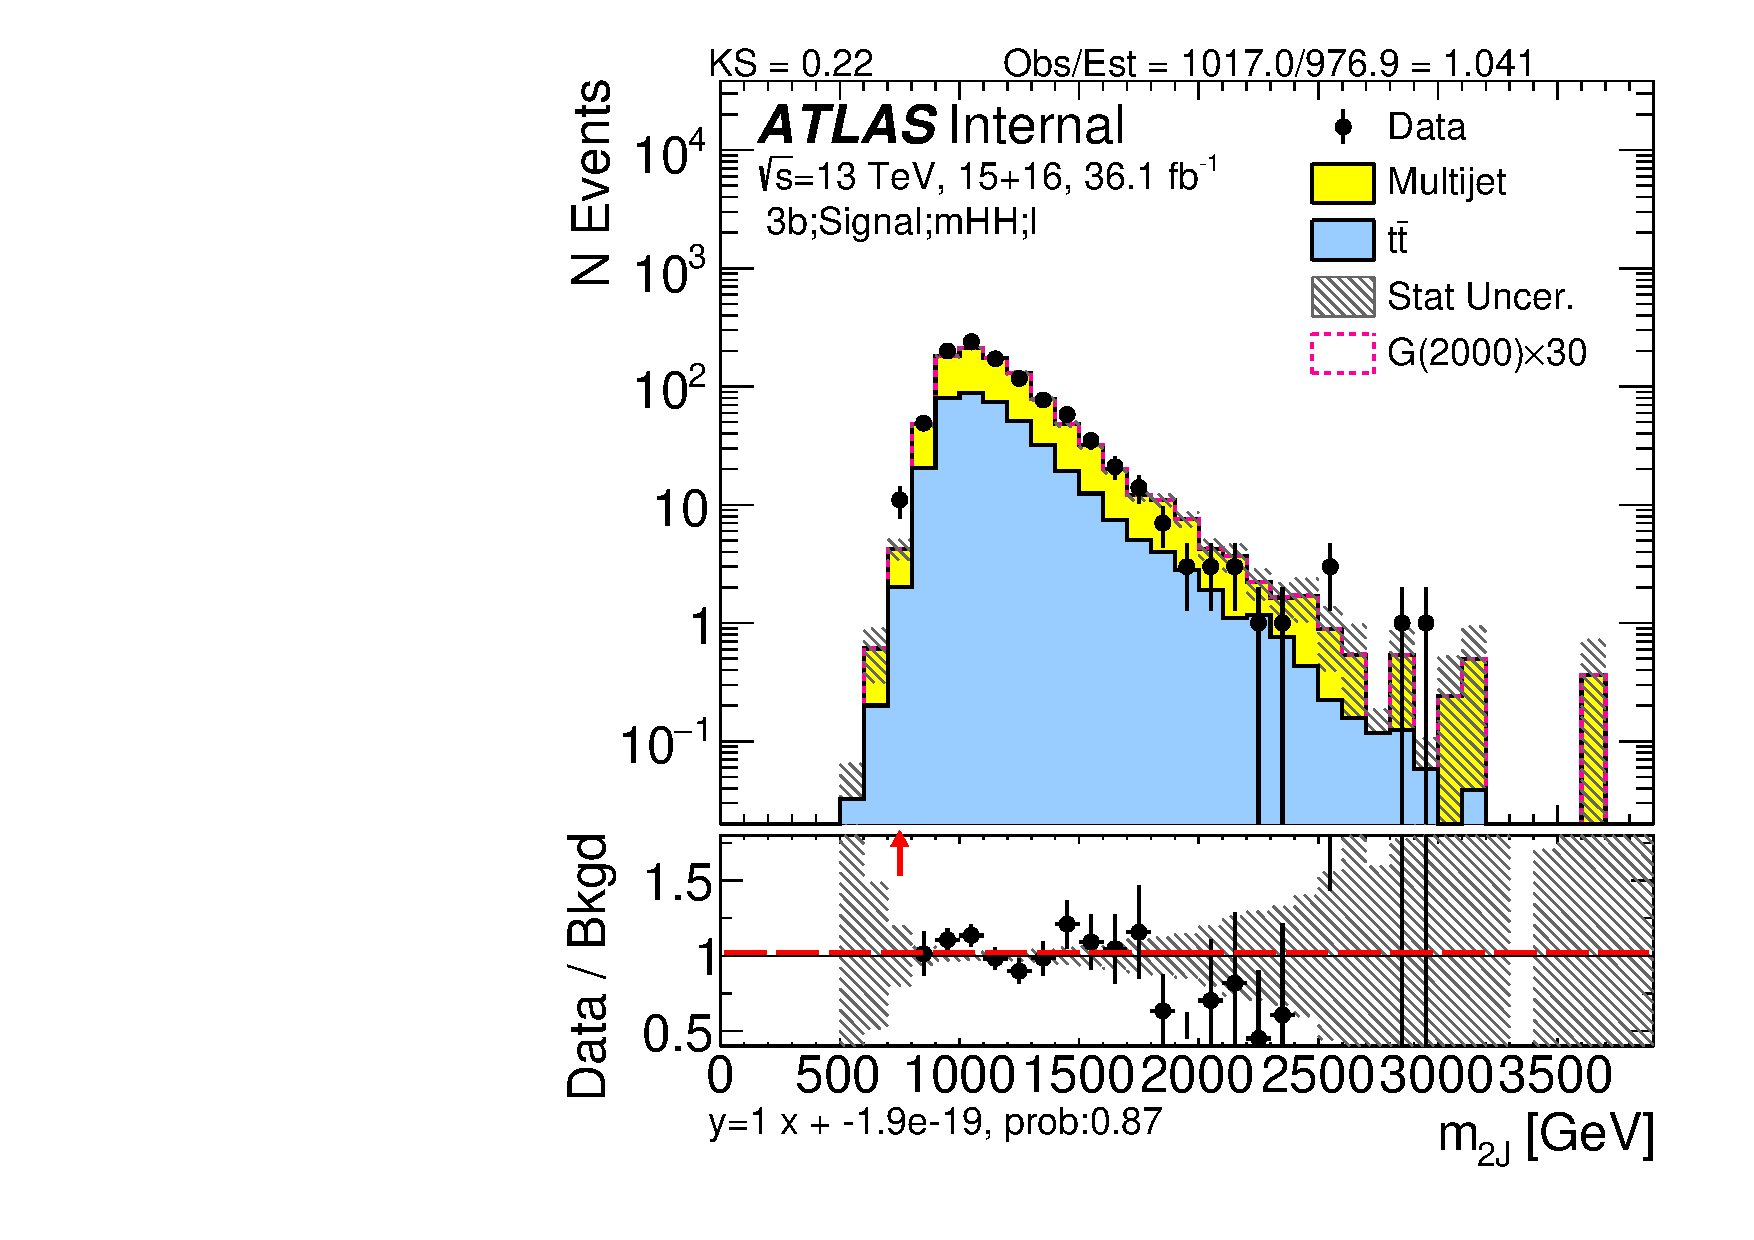
\includegraphics[width=0.45\textwidth,angle=-90]{figures/boosted/TT/Moriond_TT_ThreeTag_Signal_mHH_l_1.pdf}
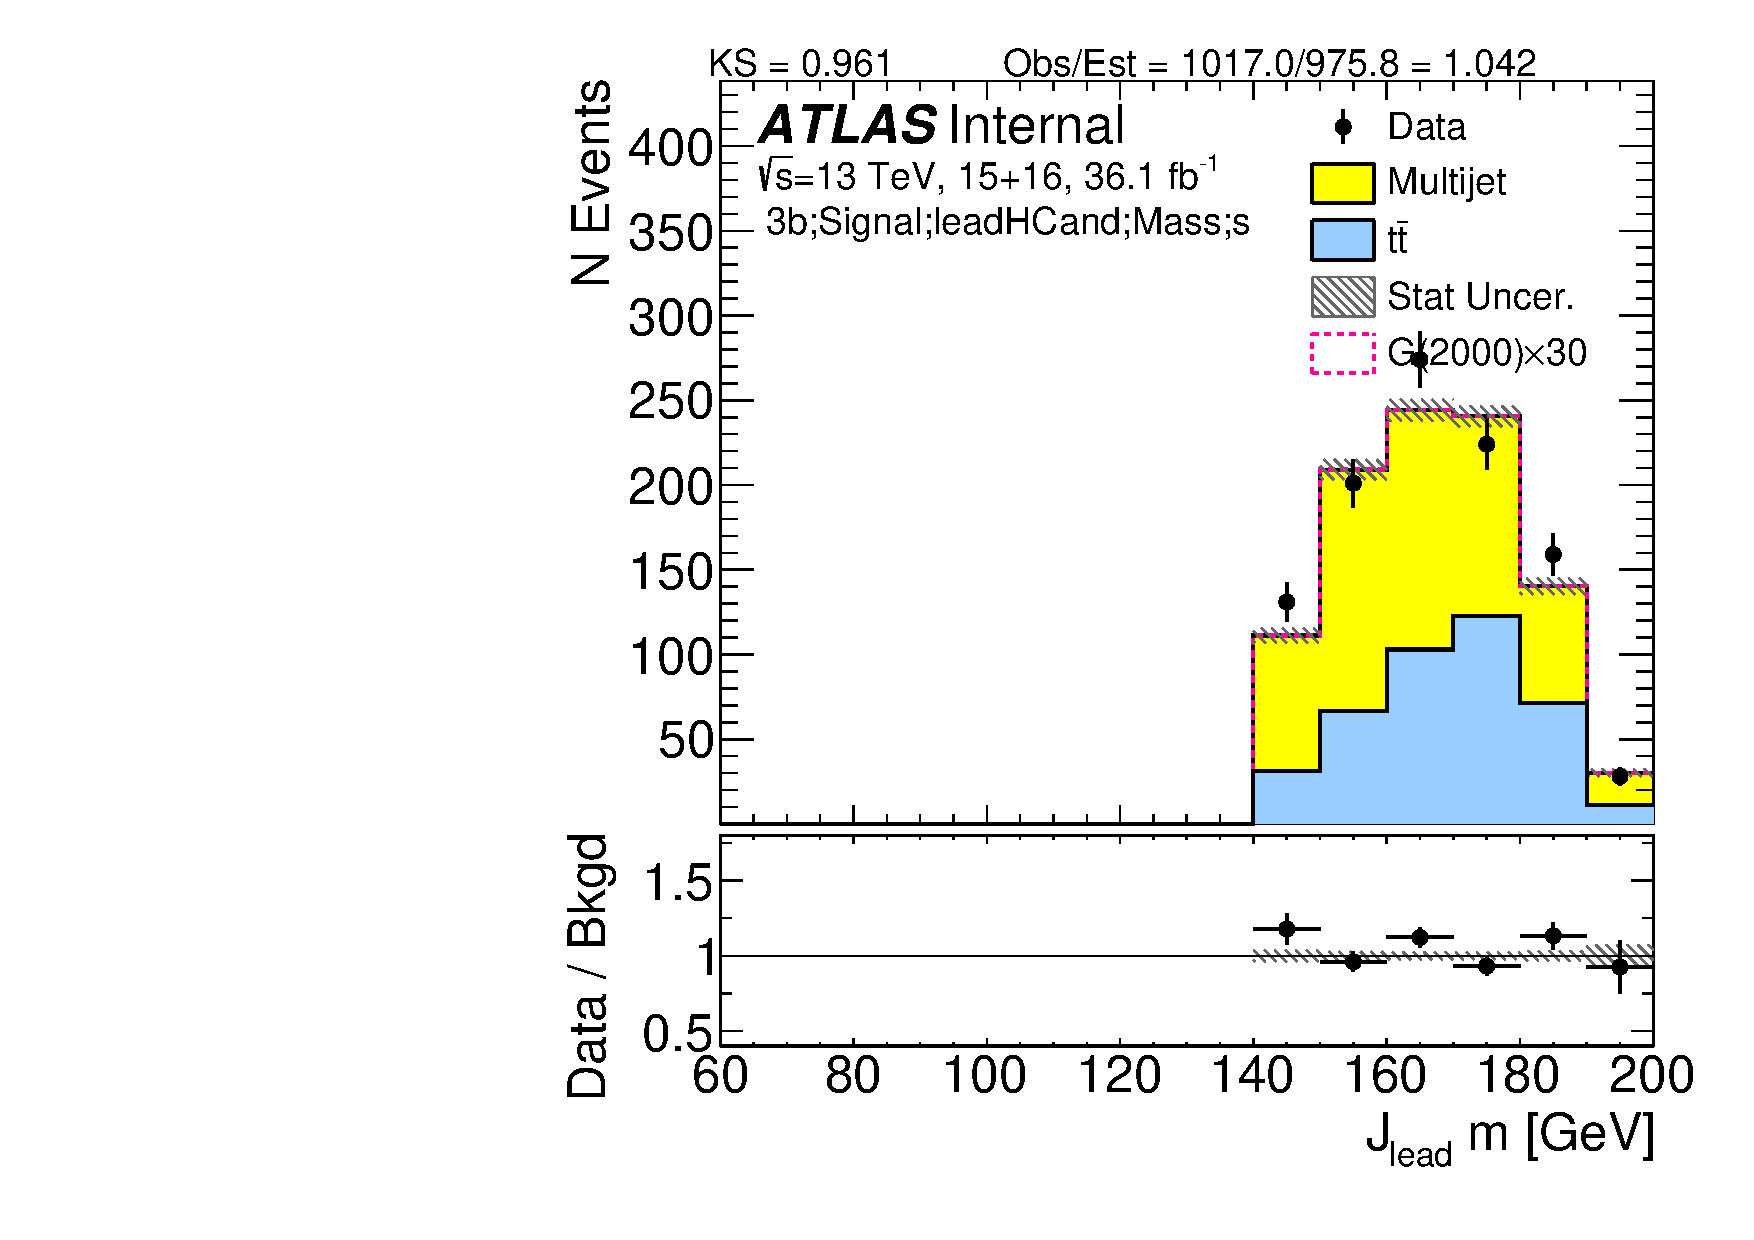
\includegraphics[width=0.45\textwidth,angle=-90]{figures/boosted/TT/Moriond_TT_ThreeTag_Signal_leadHCand_Mass_s.pdf}\\
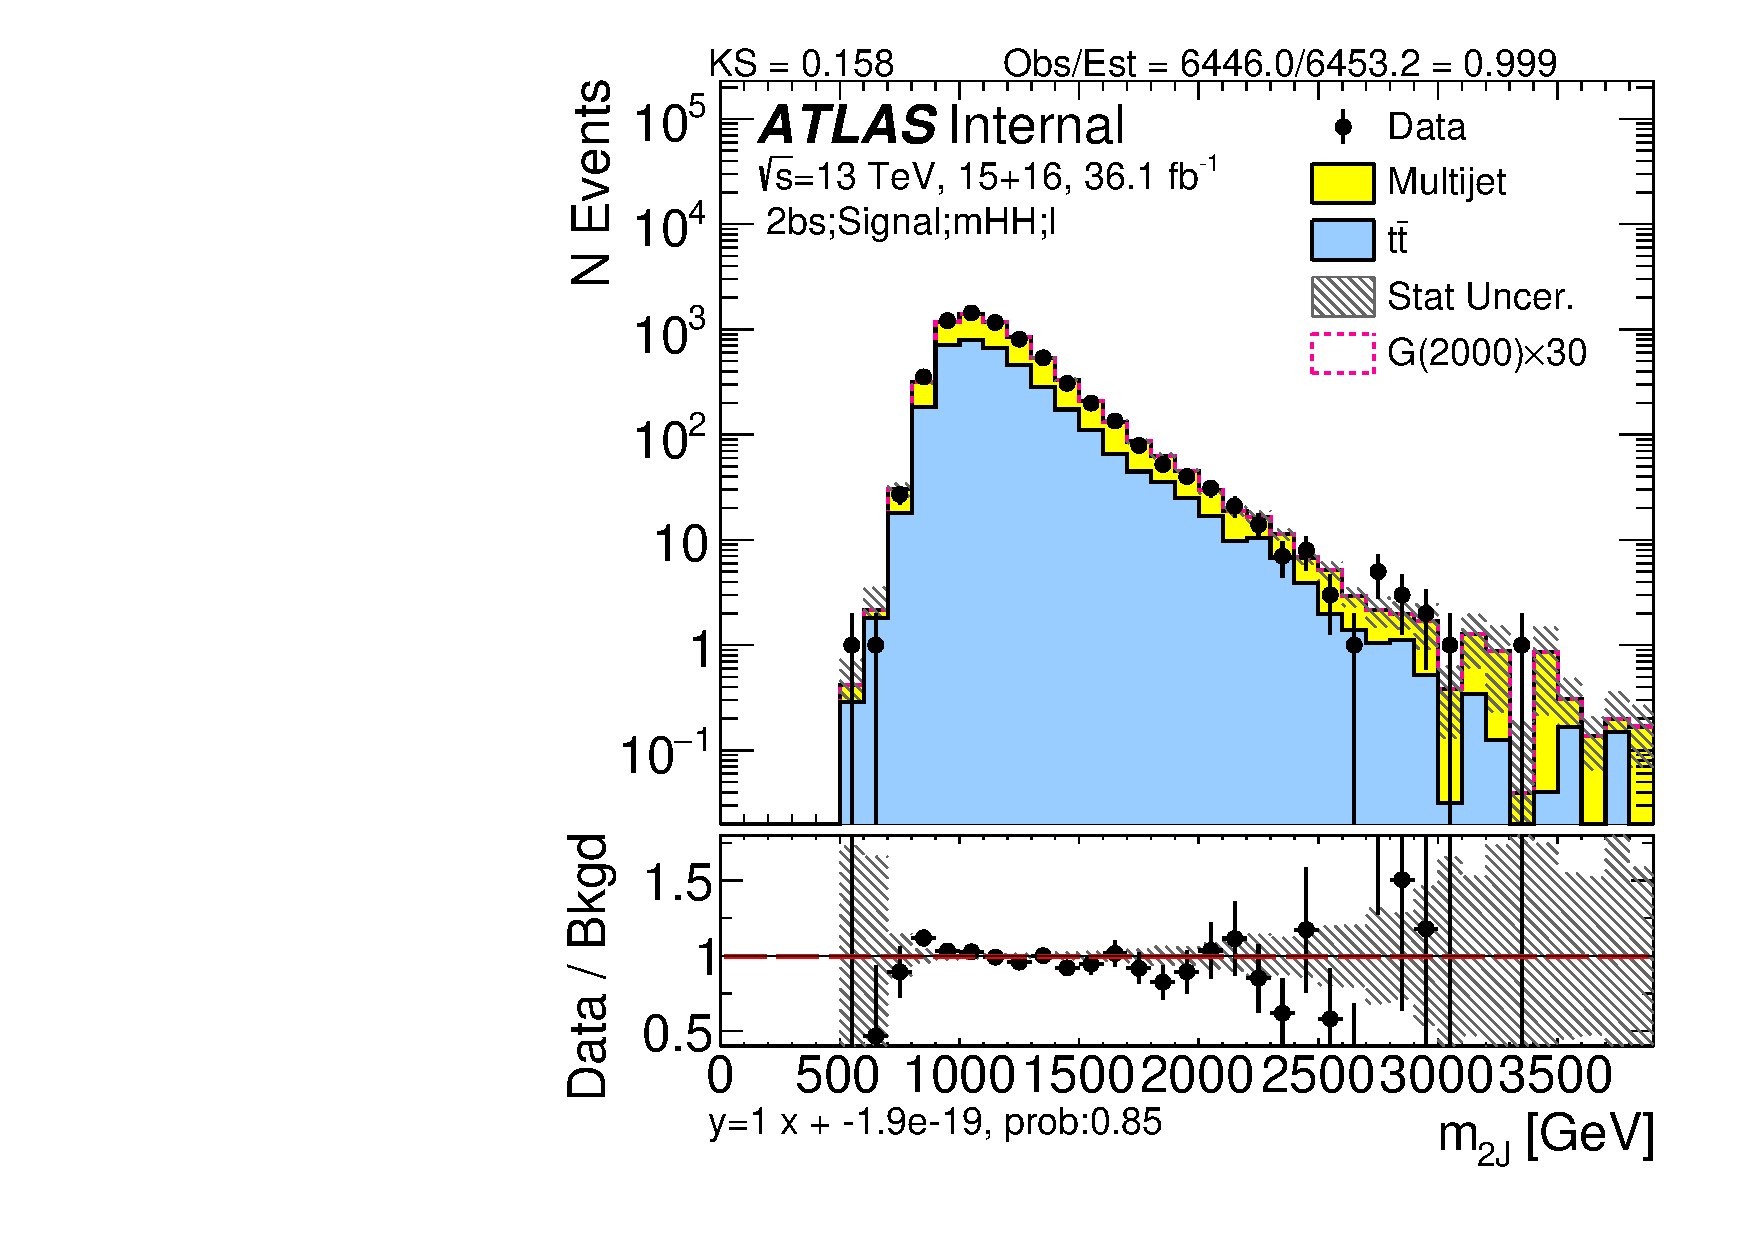
\includegraphics[width=0.45\textwidth,angle=-90]{figures/boosted/TT/Moriond_TT_TwoTag_split_Signal_mHH_l_1.pdf}
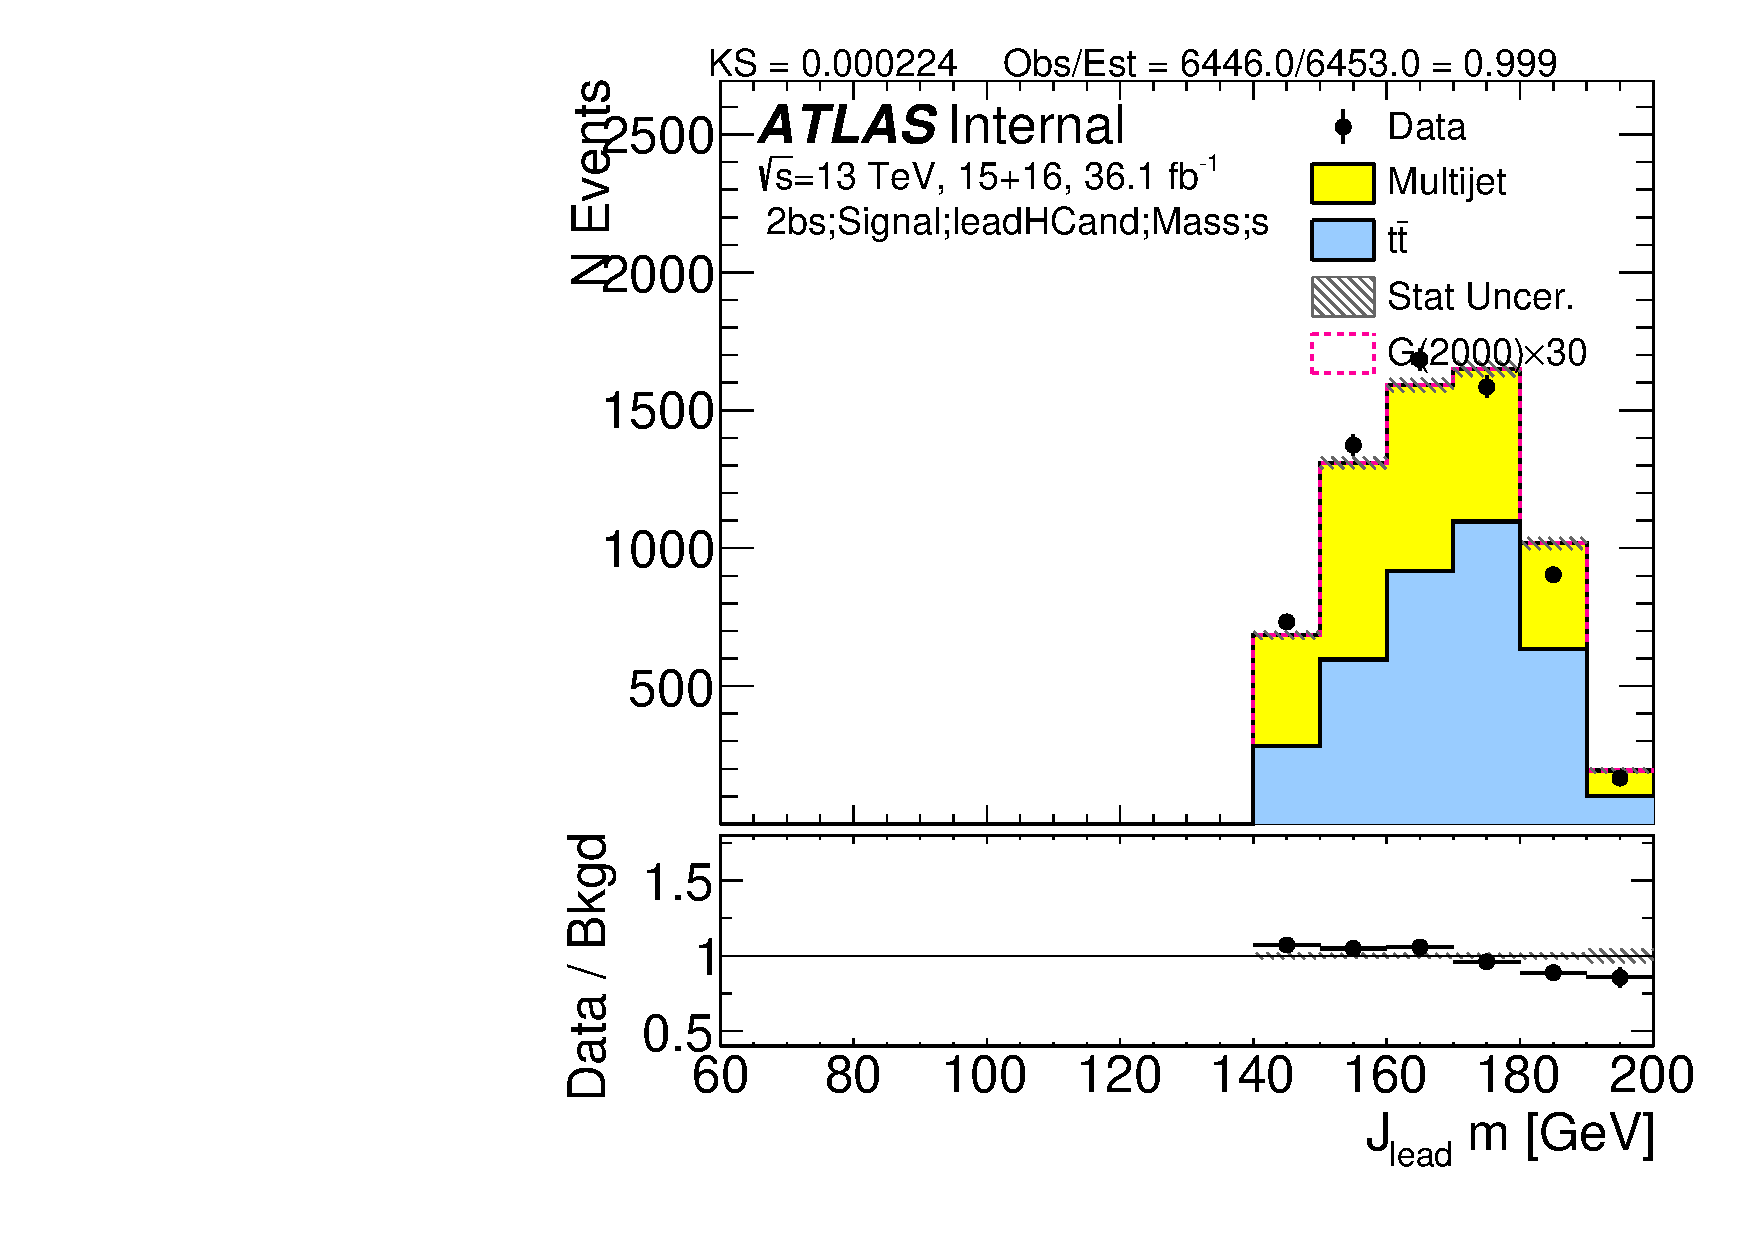
\includegraphics[width=0.45\textwidth,angle=-90]{figures/boosted/TT/Moriond_TT_TwoTag_split_Signal_leadHCand_Mass_s.pdf}\\
\end{center}
\caption{TT signal region distribution of di-jet mass (left column) and leading large-R jet mass (right column) in low mass signal, for 4$b$ (top row), 3$b$(middle row) and 2$b$ split (bottom row). The plots are with only statistical uncertainty.}
\label{CRSB:TTSR_Distribution}
\end{figure}
